\section{Worldsheet I: dictionary, inverse, moduli}
\label{ch:worldsheet-dictionary}

This chapter collects the worldsheet reading of the auxiliary fields that does not depend on a model of the inverse of the quartic form.
It starts from the first three subsections of the paper's worldsheet section before its last tightening: the auxiliary fields as groups of punctures, the inverse $\sprod{2}{2}^{-1}$ and its exclusion as a local worldsheet kernel, and the counting of moduli.
Five sections of a note on the Riemann-surface picture follow, which give the full derivations behind the dictionary: the two internal kernels, frozen-neck sewing and the chain surfaces, the coloured operad, the analogy with the $KBc$ algebra of open string field theory, and the tower of the fields $\Sigma_k$.
Four sections exist only here, written from the derivation records: the coloured grading and the Schwinger forms of the inverse together with the Neumann series, the exclusion of a sewing form for the inverse summed over levels, the geometry of the auxiliary channel after a change of its kinetic term, and the branched-cover test of the double-strand version of that change.
The chapter closes with two sections of the overview note on explicit local coordinates, the asymmetric cubic vertex with its gluings and the hyperbolic vertices, and with the figures of the Riemann-surface note.
The paper keeps a shortened version of the first three subsections; the circle picture of the inverse and the covering question are in \cref{ch:worldsheet-circle}.

\medskip

The first block opens the paper's worldsheet section and describes an auxiliary field and a $\Sigma_2$ line on the worldsheet, in the paper's notation.
The dictionary it states (fields as groups of punctures, the line of $\Sigma_2$ as two strands with no length modulus, the resolved genus as bookkeeping) is derived in full in the sections of the Riemann-surface note below, where its status is given.

\subsection{Worldsheet perspective}
\label{p:sec:worldsheet}

The cubic action is built from the string vertices of closed string field theory and from one new object, the inverse of the quartic form.
Its diagrams therefore have a worldsheet reading up to that one object, and the purpose of this section is to describe this reading.
  We first describe what an auxiliary field and a $\Sigma_2$ line are on the worldsheet, two questions that have definite answers.
  We then ask what the inverse $\sprod{2}{2}^{-1}$ can be as a surface, and what the exchange diagrams built from it correspond to on moduli space, two questions that are only partly settled.
The inverse admits, where a Neumann series converges, an algebraic representation as a series of surfaces, but no representation as a worldsheet kernel in the class defined below.
The moduli-space reading of the exchange between two quintic vertices is open.
Much of what follows is an interpretation of the algebra of \cref{p:sec:hs}.

\subsubsection{Auxiliary fields on the worldsheet}
\label{p:sec:ws:fields}

\subparagraph{Fields as surfaces.}

A vertex $\vertex{n}$ of closed string field theory is an integral over a region $\mathcal V_{0,n}$ of the moduli space of the $n$-punctured sphere, each puncture carrying one string state.
The vertices of the cubic action are the same integrals.
The coupling $\vertex{4}(\Sigma_2, \Psi^2)$ is the quartic vertex, with its region $\mathcal V_{0,4}$ and its antighost insertions, in which two of the four punctures carry the two strands of one field rather than two copies of $\Psi$.
The surface is the same, and only the grouping of the punctures changes.
A $\Sigma_n$ slot of a vertex is thus a set of $n$ punctures that belong to one field, and the state they carry is in general entangled, as the components~\eqref{p:eq:hs4:spacetime} need not be products.
We picture the punctures of a vertex as marked by the field they belong to, the two punctures of a $\Sigma_2$ slot forming one group, and we read the vertex region $\mathcal V_{0,n}$ with this marking.

\begin{figure}
  \centering
  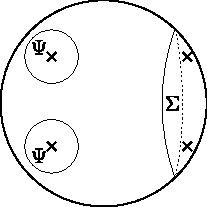
\includegraphics[width=0.3\linewidth]{V04_Psi2_Sigma.pdf}
  \caption{}
\end{figure}


A $\Sigma_n$ line of a diagram joins a $\Sigma_n$ slot of one vertex to a $\Sigma_n$ slot of another, and it carries $n$ strands, one per puncture of the slot.
Each strand is a sewing of two punctures through the inverse of the single-string pairing~\eqref{p:eq:hs1:pairing}, that is, the insertion of the level-matching bivector $b_0^- \delta_{L_0^-, 0}$ between them.
This is the sewing that produces the propagator of closed string field theory once the length of the plumbing cylinder is integrated with the insertion $b_0^+ / L_0^+$.
Here that insertion is absent: a strand is the plumbing at zero length, $w_1 w_2 = \e^{\I \theta}$, with only the twist $\theta$ integrated by the level-matching insertion, a legitimate CFT surface of measure zero in its moduli space.
A $\Psi$ line thus differs from a strand of a $\Sigma_2$ line by the integrated length alone, with its insertion $b_0^+ / L_0^+$, and not by the presence of an antighost, the level-matching insertion being common to both.
  This description holds for the pairing, and the line carries in addition the inverse $\sprod{2}{2}^{-1}$, which we discuss below.
A $\Sigma_2$ line is therefore not two strands of fixed length alone, and the surface picture of a diagram holds up to this factor.

The strands make a bookkeeping subtlety visible.
A chain of $k$ quartic vertices joined by $\Sigma_2$ lines is a tree when each line is counted as one edge, and the diagrams of \cref{p:sec:hs} are tree diagrams in this sense.
Their powers of $\gs$, their numbers of moduli and their ghost numbers are those of trees.
Resolved into punctures and strands, the same chain is the connected surface obtained by sewing $k$ spheres along $2 (k - 1)$ pairs of punctures, which has genus $k - 1$.
The two counts are reconciled by a formula that follows from the additivity of the Euler characteristic under sewing: a diagram with $L$ loops whose edges $e$ carry $k_e$ strands each has resolved genus
\begin{equation}
  \label{p:eq:ws:genus}
  g_{\mathrm{res}}
    = L + \sum_e (k_e - 1),
\end{equation}
so that a $\Sigma_2$ line raises the resolved genus by one and the loop number by zero.
No coupling and no modulus is attached to that genus, because the lengths of the necks that produce it are never integrated.
We can compare with a matrix model.
  There the double lines of a diagram fix the genus of its fat graph, and the expansion in $1 / N$ is an expansion in that genus.
  Here the strands also fix a genus, but no parameter counts it, and the physical expansion parameter $\gs$ organizes the diagrams by their loop number $L$, not by $g_{\mathrm{res}}$.

This suggests the structure of a colored operad, with one color per number of strands.
The objects are the spaces $\Hn{k}$ with their pairings $\pair[k]{\cdot}{\cdot}$.
The form $\sprod{2}{2}$ is a unary operation on the color $2$, and the cubic coupling $\vertex{4}(\Sigma_2, \Psi^2)$ is a corolla with one leg of color $2$ and two of color $1$.
Composition is the contraction of a $\Sigma_k$ line, an edge of color $k$, with the inverse of the $k$-string pairing.
The map that resolves a $\Sigma_2$ line into two ordinary strands is a linear map $\Hn{2} \hookrightarrow \Hs \otimes \Hs$ but not a map of operads, which is where the discrepancy in~\eqref{p:eq:ws:genus} comes from.
On the moduli-space side, the uncolored operad is the one of Kimura, Stasheff and Voronov on the decorated moduli spaces in which the vertex regions live~\cite{Kimura:1995:OperadStructuresModuli}.
We leave to future work the question whether the regions marked as above, together with a rule for the $\Sigma$ lines, form a colored operad of moduli spaces.
The obstacle is the line itself: its composition is not given by any kernel of the class defined below, and the one surface representation known, the Neumann series, carries algebraic factors.



The second block holds the paper's subsections on the inverse of the quartic form and on the counting of moduli.
It states three results:
\begin{itemize}
  \item there is no local worldsheet kernel for $\sprod{2}{2}^{-1}$, an exclusion within connected surfaces of bounded type carrying standard sewing ghost insertions (any genus, any number of vertices and frozen nodes, smoothed handles, continuous moduli with their $b$-ghost measure), modulo the standard input that these are the only insertions at a degenerating node: \status{Proven}\record{022-rs5-no-local-kernel-theorem (R28)};
  \item the Neumann series is a representation of $\sprod{2}{2}^{-1}$ as a convergent sum over chains of frozen-neck surfaces, under the hypothesis that the spectral radius of the iterated operator is smaller than one for the level-diagonal split, away from the zeros of the truncated determinant (\cref{ch:hypotheses}): \status{Conditional(PH21) -- Proven}\record{020-riemann-m2-geometric (R27)};
  \item the virtual dimensions of the calculus with negative moduli, for every number of punctures on the sphere, and their closure at every order: \status{Proven}\record{036-covering-m06-composite (R59)}.
\end{itemize}
The finite-model demonstration that the Neumann series can converge or diverge, while the algebraic inverse telescopes in both cases, is written out in \cref{sec:ws1:neumann}.

\subsubsection{The inverse of the quartic form}
\label{p:sec:ws:inverse}


The propagator of the auxiliary field is the inverse of a vertex, and we now ask what it means in the worldsheet description.
The propagator of the string field in Siegel gauge contains the operator $1 / L_0^+$wich can be written as a Laplace transform:
\begin{equation}
  \label{p:eq:ws:propagator-psi}
  \frac{1}{L_0^+}
    = \int_0^\infty \dd s \; \e^{- s L_0^+},
\end{equation}
This representation gives the worldsheet computation.
The operator $\e^{- s L_0^+}$ is a cylinder of length $s$, the integral over $s$ is the integral over the length of the plumbing cylinder, and $b_0^+$ is the antighost insertion that goes with that modulus.
The spectrum of $L_0^+$ is not positive, because of the tachyon, so that the RHS~\eqref{p:eq:ws:propagator-psi} does not converge, strictly speaking.
However, the LHS is perfectly well-defined and can be used as a \emph{definition} of the RHS whenever the latter is not~\cite{Sen:2015:OffshellAmplitudesSuperstring,deLacroix:2017:ClosedSuperstringField,Erbin:2021:StringFieldTheory}.

In the same spirit we write
\begin{equation}
  \label{p:eq:ws:propagator-sigma}
  \sprod{2}{2}^{-1}
    = \int_0^\infty \dd t \; \e^{- t \sprod{2}{2}},
\end{equation}
on the quotient where $\sprod{2}{2}$ is invertible, the left-hand side being the object the cubic action defines.
Making sense of the exponent needs one choice: a real positive inner product on the truncated $2$-string space, which identifies the two ghost-number sectors that the quartic form connects.
The representation~\eqref{p:eq:ws:propagator-sigma} needs in addition a sign condition on the spectrum of the quartic form in that inner product, a condition the quartic form need not satisfy.
The alternative representation $\int_0^\infty \dd t \, A \, \e^{- t A^2}$, with $A$ the real symmetric matrix of the quartic form in an orthonormal basis of that inner product, needs no such condition.
The inner product enters the integrand but not the result.
We keep the representation~\eqref{p:eq:ws:propagator-sigma} for the comparison with~\eqref{p:eq:ws:propagator-psi}, since its exponent is the quartic form itself.
  The conclusion of the next paragraph holds for the alternative as well, whose integrand expands in chains of an odd number of vertices and not term by term in the propagator.

The representation differs from~\eqref{p:eq:ws:propagator-psi} by its exponent.
In~\eqref{p:eq:ws:propagator-sigma} the exponent is the quartic form itself: there is no $L_0^+$, no $b_0^+$, and the parameter $t$ is not the length of anything.
Expanded in powers of $t$, the integrand $\e^{- t \sprod{2}{2}}$ at fixed $t$ is a sum over chains of quartic vertices joined through the inner product chosen above, which identifies the two ghost-number sectors, with the weight $(- t)^k / k!$ for the chain of $k$ vertices.
In surfaces these are chains of four-punctured spheres sewn along necks of fixed length.
The parameter $t$ is a spectral variable conjugate to the vertex, and the integral over $t$ does not commute with the expansion: each term $\int_0^\infty t^k \, \dd t$ diverges.
The representation~\eqref{p:eq:ws:propagator-sigma} therefore does not provide a term-by-term expansion of the propagator in surfaces, in contrast with~\eqref{p:eq:ws:propagator-psi}, whose integral over $s$ is part of the integral over the moduli of the sewn surface.

A representation that does expand in surfaces is the Neumann series.
Split the quartic form into its level-diagonal part and the rest,
\begin{equation}
  \label{p:eq:ws:neumann}
  \sprod{2}{2}
    = D - R,
  \qquad
  \sprod{2}{2}^{-1}
    = \sum_{k \ge 0} (D^{-1} R)^k \, D^{-1},
\end{equation}
with $D$ invertible on the quotient.
The series converges when the spectral radius of $D^{-1} R$ is below one, which we assume (and motivate below).
The term of order $k$ is a chain of $k$ insertions of $R$, the level-off-diagonal part of the quartic vertex, threaded on $k + 1$ level-diagonal $\Sigma_2$ lines $D^{-1}$.
In surfaces it is a chain of $k$ four-punctured spheres sewn pairwise along two necks of fixed length, each $\Sigma_2$ line, internal or external, carrying one algebraic factor $D^{-1}$ on its level, which acts on its pair of necks, and each sphere carrying the projection that removes the level-diagonal part of its vertex.
Where the series converges, this gives $\sprod{2}{2}^{-1}$ in terms of Riemann surfaces, up to the algebraic factors $D^{-1}$, which are not surfaces.
It is a sum over a discrete family of chains of surfaces with necks of fixed length, one algebraic factor per $\Sigma_2$ line and per vertex, rather than an integral over a continuous family.
The split~\eqref{p:eq:ws:neumann} is a choice, like a subtraction scheme, but the sum does not depend on it when it converges.
For example, for the quartic $\mathrm{SL}(2, \C)$ vertex~\cite{Erbin:2023:SL2CQuarticVertex,Erbin:2026:SL2CVerticesClosed}, on the block of pairs of zero-momentum tachyons and ghost dilatons, the spectral radius of $D^{-1} R$ is below one at the two values of the stub parameter $\beta$ checked, so the series converges there.
The matrix is not diagonally dominant on this block: the radius is below one because the products of off-diagonal entries partly cancel.
At other momenta and on the other blocks the convergence is open.
The series in $\gs$ of \cref{p:sec:hs:quintic}, which dresses $\sprod{2}{2}^{-1}$ with quintic vertices, is a Neumann series of the same kind, and its terms are chains of the same kind with quintic vertices on the line.

We can ask whether the propagator can instead be a worldsheet kernel of the usual kind, as $b_0^+ / L_0^+$ is.
By a kernel of the usual kind we mean an integral, over a finite-dimensional parameter space with a signed measure, of ghost-dressed correlators on connected surfaces with four external punctures, two in and two out.
The surfaces may have any genus and any number of nodes, the topology staying bounded over the parameter space.
They carry one antighost insertion per integrated modulus and, at each node, the standard sewing insertion: $b_0^- \delta_{L_0^-, 0}$ for a node of fixed length and $b_0^+ b_0^- / L_0^+ \, \delta_{L_0^-, 0}$ for a node whose length is integrated.
The class contains every finite connected chain of spheres sewn along necks, with the moduli of the spheres integrated or not.
The double tube, two independent plumbing cylinders, is disconnected and lies outside it.
No kernel of this class equals $\sprod{2}{2}^{-1}$, by ghost-number counting.
The inverse lowers the ghost number by two, as $\sprod{2}{2}$ raises it by two, while every correlator of the class raises it by at least two:
\begin{equation}
  \label{p:eq:ws:ghost-obstruction}
  \Ngh\big( \sprod{2}{2}^{-1} \big)
    = - 2,
  \qquad
  \Ngh\big( \text{kernel} \big)
    = 2 + \nu_f + m
    \ge 2,
\end{equation}
where $\nu_f$ is the number of nodes of fixed length and $m$ the number of unintegrated real moduli.
The second count rests on the standard factorization of CFT correlators at a node, which fixes the insertion there to the ones listed.
This is the one input of the argument, and we take it from~\cite[ch.~9]{Polchinski:2005:StringTheoryVolume} without rederiving it.
Within the class so defined the exclusion is a proof by counting, and it says nothing outside it: the insertions that could lower the ghost number, antighosts attached to no modulus, are those the class leaves out, and they are the subject of the second option below.

Outside the class lie, among others, three options.
The first is the Neumann series~\eqref{p:eq:ws:neumann}, an infinite sum with one algebraic factor per $\Sigma_2$ line and per vertex.
The second is a dressing of the surfaces by such insertions, tuned to the actual quartic vertex.
  A dressing built uniformly from the vertex data, the same construction for every vertex, is excluded by its degree: under a rescaling $\vertex{4} \to t \, \vertex{4}$ of the vertex it is homogeneous of non-negative degree in $t$, while $\sprod{2}{2}^{-1}$ has degree $- 1$.
  A dressing at the actual vertex data is not excluded by this argument.
The third is a change of the kinetic term of the auxiliary field, which is what the construction of~\cite{Erbin:2024:OpenStringStub} does for the stub of an open string field theory.
This changes the identity to be satisfied rather than the kernel.
The reading of a $\Sigma_2$ line as a surface in the previous paragraphs holds up to this one factor, which is algebraic.

\subsubsection{Counting moduli}
\label{p:sec:ws:moduli}

If a $\Sigma_2$ line carries no modulus, a diagram with such lines has fewer moduli than the vertices it is made of.
The count nevertheless matches, at every order, the dimension of the moduli space that the diagram would have to cover.
We assign to every vertex the real dimension of its region, $\hat d(\vertex{n}) = \dim_\R \mathcal V_{0,n} = 2 n - 6$, the dimension of the moduli space of the $n$-punctured sphere, extended to $n \le 2$ by the same formula.

Kinetic operators count as the vertices they are, $\hat d(Q_B) = \hat d(\vertex{2}) = - 2$ and $\hat d(\sprod{2}{2}) = \hat d(\vertex{4}) = + 2$, and the count is additive under gluing.
The dimension assigned to an inverse is then minus that of what it inverts.
For the string field this gives $\hat d(Q_B^{-1}) = + 2$, the two real moduli of the plumbing cylinder: its length, integrated with $b_0^+ / L_0^+$, and its twist, integrated by the level-matching insertion $b_0^- \delta_{L_0^-, 0}$ of the pairing.

A handle of the resolved surface~\eqref{p:eq:ws:genus} counts $- 6$, the shift of the ghost-number anomaly: $\hat d$ is the number of antighost insertions minus the number of ghost insertions minus six per resolved handle, and on a connected tree the number of integrated real moduli.
For the auxiliary field it gives
\begin{equation}
  \label{p:eq:ws:negative-moduli}
  \hat d\big( \sprod{2}{2}^{-1} \big)
    = - 2,
\end{equation}
two moduli removed rather than added.
This is the dimension-counting form of the ghost-number mismatch~\eqref{p:eq:ws:ghost-obstruction}, the two gradings agreeing on $\sprod{2}{2}$ and its inverse, and it is the sense in which a $\Sigma_2$ line carries negative moduli.
With it the count closes at every order:
\begin{equation}
  \label{p:eq:ws:closure}
  \begin{aligned}
    \hat d\big( \vertex{4} \, \sprod{2}{2}^{-1} \, \vertex{4} \big)
      &
      = 2 - 2 + 2
      = 2
      = \dim_\R \mathcal M_{0,4},
    \\
    \hat d\big( \vertex{4} \, \sprod{2}{2}^{-1} \, \vertex{5} \, \sprod{2}{2}^{-1} \, \vertex{4} \big)
      &
      = 2 - 2 + 4 - 2 + 2
      = 4
      = \dim_\R \mathcal M_{0,5},
    \\
    \hat d\big( \vertex{5} \, \sprod{2}{2}^{-1} \, \vertex{5} \big)
      &
      = 4 - 2 + 4
      = 6
      = \dim_\R \mathcal M_{0,6},
  \end{aligned}
\end{equation}
and the same closure holds for the longer chains, whose count reduces to $2 N - 6$ for $N$ external legs.
The diagrams of the cubic theory have, formally, the dimension of the moduli space with their number of external punctures, as the diagrams of closed string field theory do.
The $\Psi$-channel analogue is $\hat d(\vertex{3} \, Q_B^{-1} \, \vertex{3}) = 0 + 2 + 0 = 2$, the familiar statement that the $3$-string vertex and the propagator together have the moduli of the four-punctured sphere.
These are corollaries of the additivity of the count under gluing, and they are the same statement as the saturation of the ghost number on the sphere.

The count is necessary for a geometric reading and never sufficient, as two facts show.
The four-point chain $\vertex{4} \, \sprod{2}{2}^{-1} \, \vertex{4}$ has the dimension of $\mathcal M_{0,4}$, and it equals $\vertex{4}$ by the collapse~\eqref{p:eq:hs4:telescoping}: a chain that is a single vertex region, covering only $\mathcal V_{0,4}$.
The dimension count is satisfied there because the line removes exactly the two moduli that the second vertex region would have added, which is how the collapse shows in the count.
Conversely, the double tube, two plumbing cylinders whose lengths and twists are integrated independently, is a bona fide family of surfaces with the same count $\hat d = - 2$, and it is not the inverse.
With any signed measure over its two lengths and twists, it commutes with the two operators $L_0^\pm$ of the strands and is therefore diagonal in the $2$-string level, while $\sprod{2}{2}$ has a non-vanishing level-off-diagonal part $R$ and so has its inverse.
This excludes the double tube.
Being disconnected, it lies outside the class of~\eqref{p:eq:ws:ghost-obstruction}, whose count alone does not exclude it.

The count does not single out a surface either.
The double tube of the previous paragraph reaches $\hat d = - 2$ by the handle rule, its two cylinders sitting at resolved genus one, with no $c$-ghost insertion.
A connected surface reaches $\hat d = - 2$ only with antighost insertions attached to no modulus of its own surface, the zero modes of plumbing fixtures on its external legs, which the class of~\eqref{p:eq:ws:ghost-obstruction} does not admit.
Sewn into a diagram, they become the moduli of the two resolved handles, which is how the handle rule reaches $- 2$.
Such dressings are excluded only as uniform constructions, as said above.
A negative formal dimension is therefore not by itself an obstruction to a geometric reading, as $2$-strand families reach it through a handle.
The obstruction is the ghost-number argument~\eqref{p:eq:ws:ghost-obstruction} for connected surfaces with the standard insertions of its class, and level-diagonality for the disconnected double tube.

At six points the count is the first that is not explained by a collapse.
The composite vertex $\vertex{5 \cdot 5}$ of~\eqref{p:eq:hs5:exchange-vertex} has the dimension of $\mathcal M_{0,6}$, and it is the first chain whose line joins two interaction vertices, so that it does not collapse by the criterion of \cref{p:sec:hs:sextic:kernel}.
We call \emph{covering question} the question whether it covers a region of $\mathcal M_{0,6}$, and covers it once.
  We return to it below, after the circle picture has given the line a geometric model.
Everything in this counting is bookkeeping at a fixed level of truncation and at tree level: it gives the dimensions and says nothing about the regions themselves.



\medskip

\noindent
The next five blocks come from a note on the Riemann-surface picture of the auxiliary sector.
It derives the dictionary that the paper's worldsheet section summarizes, with the ghost-saturation diagnostic, the frozen-neck definitions, the three-grading table and the genus formula of the coloured operad.
Its results, and their status:
\begin{itemize}
  \item the two internal kernels distinguished, frozen-neck chains and their gradings, the combinatorial covering by the three exchange channels, the genus formula $g_{\rm res} = L_c + \sum_e (k_e - 1)$ of the coloured operad: \status{Proven}\record{020-riemann-m2-geometric (R27)};
  \item the identification of one contraction with the inverse single-string pairing as plumbing at frozen length, $\omega_1^{-1} = b_0^- \delta_{L_0^-, 0}$, and the factorized propagator $(b_0^+ / L_0^+) \, \omega_1^{-1}$: \status{Verified}\record{021-rs4-sewing-fixtures (R27)};
  \item the Laplace and Schwinger forms of $\sprod{2}{2}^{-1}$, under spectral conditions that are open beyond level~$0$: \status{Conditional(PH1) -- Proven} (\cref{sec:ws1:schwinger});
  \item the dictionary with the $KBc$ algebra of open string field theory is an organizing analogy, not a result, and carries no status.
\end{itemize}
The note uses an earlier notation, translated below.

\begin{quote}
  \small
  \textbf{Translation box: Riemann-surface note $\to$ paper.}
  \begin{itemize}
    \setlength{\itemsep}{0.3ex}
    \item $V_n$ $\to$ $\vertex{n}$; $V_4$ read as a bilinear form on $\Sym^2 \Hilb_0$ is the paper's $\vertex{4}(A, B) = \pair[2]{A}{\sprod{2}{2}(B)}$, and $V_4(\Sig, \Sig)$ is the kinetic term of $\Sigma_2$.
    \item $\mtwo = G_2^{-1} V_4$ $\to$ $\sprod{2}{2}$; $\mtwo^{-1}$ $\to$ $\sprod{2}{2}^{-1}$; $\Ngh(\mtwo) = + 2$ is the physical ghost number of $\sprod{2}{2}$.
    \item $\Hilb_0$ $\to$ $\Hs$ restricted to level-matched states; $\Sym^k \Hilb_0$ $\to$ $\Hn{k}$; $G_k = \omega_1^{\otimes k}$ $\to$ the multi-string pairing $\pair[k]{\cdot}{\cdot}$; $\Sig \equiv \Sigma_2$, $\Sig_k \to \Sigma_k$.
    \item The two kernels: the \enquote{worldsheet sewing kernel} $\mathsf P$ of a colour-1 line is the propagator of $\Psi$; the \enquote{colour-2 contraction} $\mathsf S = (12 / \gs^2) \, \mtwo^{-1} G_2^{-1}$ is the propagator of $\Sigma_2$ of the Feynman rules (\cref{p:sec:hs:quartic}).
    \item HS (Hubbard--Stratonovich) Feynman rules are the Feynman rules of the cubic action; $\pklg$ are the maps of the IBL structure of \cref{ch:ibl}.
    \item In the tower section, $\tilde V_{2k}(\Sig_k, \Sig_k)$ is the kinetic term of $\Sigma_k$ built from the reduced vertex, $\dvertex{2k}(\Sigma_k, \Sigma_k) = \pair[k]{\Sigma_k}{\wprod{k}{k}(\Sigma_k)}$ (\cref{ch:all-orders}); the symbols $\hat M_k$, $\hat H_k$, $L_k$ of the continued fraction are the note's own.
    \item \emph{Reality.} The note's conjugation is $\ddagger = (-1)^{\Ngh + 1} \star$ on each strand, so that its condition $\Sig_k^\ddagger = \Sig_k$ is the paper's $\Sigma_k^\star = (-1)^k \Sigma_k$: the two read the same for $\Sigma_2$, while for odd $k$ the sign is explicit, $\Sigma_3^\star = - \Sigma_3$, and $\Psi^\ddagger = \Psi$ is $\Psi^\star = - \Psi$ (\cref{ch:conventions}).
  \end{itemize}
\end{quote}

The first section of the note separates the two internal lines of a diagram, the propagator of $\Psi$ and the contraction of $\Sigma_2$, by the count of one $b$-ghost per real modulus.

\subsection{The two internal kernels}
\label{rs:sec:kernels}

The whole geometric story turns on keeping apart two objects that both look like
``an internal line'' in a Feynman graph but are worldsheet-geometrically
opposite. This section defines them and gives the sharp diagnostic --- one
$b$-ghost per real modulus --- that tells them apart.

\subparagraph{Vertices are moduli integrals; ghost saturation is the bookkeeping.}
A closed-string vertex is an integral over a vertex region of a fixed-surface
correlator with one $b$-ghost insertion per real modulus,
\begin{equation}
	V_4(A_1,\dots,A_4)
	= \int_{\mc{V}_{0,4}}\!\dd^2 m\;
	\Bra{\Sig_{0,4}(m)}\,b(v_m)\,b(\bar v_m)\,
	\ket{A_1}\otimes\cdots\otimes\ket{A_4},
	\label{rs:eq:V4integral}
\end{equation}
where $\Bra{\Sig_{0,4}(m)}$ is the four-punctured-sphere surface state at moduli
point $m$ with its chosen local coordinates, and each $b$ soaks up one real
modulus. A sphere correlator is non-zero only when the total ghost number
saturates the background charge: it needs $\Ngh=6$, and each $b$ costs one unit,
so a genus-zero $n$-point vertex on its region ($\dim_\R=2(n-3)$) is non-zero iff
\begin{equation}
	\sum_i \Ngh(A_i) \;=\; 6 + 2(n-3).
	\label{rs:eq:saturation}
\end{equation}
This is the precise sense in which \emph{one $b$-insertion per real modulus} is
the sharp diagnostic for ``is this parameter a modulus''. Every elementary vertex
of the construction saturates \eqref{rs:eq:saturation} identically, at every level
of the tower; \Cref{rs:tab:saturation} lists them. \emph{(Terminology note, sharpened
by the comparison with the closed-string sewing conventions of~\cite{Erbin:2021:StringFieldTheory}: the $b(v_m),b(\bar v_m)$ here are the Schiffer-vector
insertions soaking up a \emph{vertex-region} modulus $m$; they are distinct from
the propagator zero-modes $b_0^\pm$ of \Cref{rs:sec:frozen}. The two diagnostics
agree on the discriminant that matters: only a \emph{length}-type modulus needs a
compensating $b$; the level-matching $b_0^-\delta_{L_0^-,0}$ retained by every
frozen-neck contraction is not itself a modulus and needs no partner.)}

\begin{table}[htp]
	\centering
	\begin{tabular}{lcccc}
		\toprule
		vertex & fields ($\Ngh$ each) & $\sum\Ngh$ & $\#b = \dim_\R$ region & $\sum\Ngh-\#b$ \\
		\midrule
		$V_4(\Sig,\Sig)$ & $4,4$ & $8$ & $2$ & $6$ \\
		$V_4(\Sig,\Psi,\Psi)$ & $4,2,2$ & $8$ & $2$ & $6$ \\
		$\tilde V_{2k}(\Sig_k,\Sig_k)$ & $2k,2k$ & $4k$ & $2(2k-3)$ & $6$ \\
		$\tilde V_{2k+1}(\Sig_k,\Sig_k,\Psi)$ & $2k,2k,2$ & $4k+2$ & $2(2k-2)$ & $6$ \\
		\bottomrule
	\end{tabular}
	\caption{Ghost saturation \eqref{rs:eq:saturation} for every elementary vertex of
	the construction (the $\Ngh$ assignments are the physical ghost numbers of the products; the region
	dimensions are the standard $\dim_\R\mc{V}_{0,n}=2(n-3)$). Each row balances to
	$6$: the vertices are \emph{bona fide} moduli integrals with exactly the right
	number of $b$-insertions. This table is the diagnostic used repeatedly below:
	an internal line carries a modulus iff adding it would spoil the balance unless
	accompanied by its own $b$.}
	\label{rs:tab:saturation}
\end{table}

\subparagraph{Kernel 1: the worldsheet sewing kernel (colour-1 line).} An ordinary
closed-string internal line sews two surface states by inserting a complete set
of states weighted by the plumbing factor and integrated with the $b$-ghost
measure:
\begin{equation}
	\mathsf P
	= \int_0^\infty\!\dd s\int_0^{2\pi}\!\frac{\dd\theta}{2\pi}\;
	b_0^+\,b_0^-\;\e^{-sL_0^+ + \I\theta L_0^-}
	= \frac{b_0^+\,b_0^-}{L_0^+}\,\delta_{L_0^-,0}
	= \frac{b_0^+}{L_0^+}\,\omega_1^{-1}
	\label{rs:eq:sewing}
\end{equation}
(normalisation \textbf{verified exact} against Erbin's conventions \cite{Erbin:2021:StringFieldTheory}
including the plumbing-integral prefactor; the
factorised form separates the length-modulus factor $b_0^+/L_0^+$ from the
level-matching sewing measure $\omega_1^{-1}=b_0^-\delta_{L_0^-,0}$, identified
precisely in \Cref{rs:sec:frozen}). The point is geometric, not formal: the operator
$e^{-sL_0^+}$ \emph{is} a surface --- the CFT path integral on a flat cylinder of
length $s$ and twist $\theta$ --- and \emph{each} value of $(s,\theta)$ is a
\emph{different} surface. The double integral sweeps a two-real-parameter family
inside moduli space, and correspondingly the kernel carries exactly two
$b$-insertions, $b_0^+$ and $b_0^-$. This is how the $s$-, $t$- and $u$-channel
Feynman graphs sweep out the three propagator regions
$\mc{M}_s,\mc{M}_t,\mc{M}_u\subset\mc{M}_{0,4}$.

\subparagraph{Kernel 2: the colour-2 contraction (colour-2 edge).} Between two
$V_4(\,\cdot\,;\Psi,\Psi)$ vertices the HS Feynman rules (\cref{p:sec:hs:quartic}) insert the
\emph{state-space} kernel
\begin{equation}
	\mathsf S
	= \frac{12}{\gs^2}\,\big(V_4|_{\Sym^2}\big)^{-1}
	= \frac{12}{\gs^2}\,\mtwo^{-1}\,G_2^{-1},
	\label{rs:eq:Skernel}
\end{equation}
where $V_4|_{\Sym^2}$ is the restriction of the quartic vertex to the symmetric
square and the inverse is taken with respect to the symmetric identity. Read it
against \eqref{rs:eq:sewing}: there is \textbf{no} plumbing parameter $q$, \textbf{no}
$s$-integral, \textbf{no} \emph{length-modulus} insertion $b_0^+/L_0^+$, and
\textbf{no} $L_0^+$ (the level-matching sewing measure
$\omega_1^{-1}=b_0^-\delta_{L_0^-,0}$ \emph{per strand} is retained --- see
\Cref{rs:sec:frozen} --- it is not a length modulus). It is the inverse
of an object \eqref{rs:eq:V4integral} whose moduli have \emph{already} been
integrated. That single fact --- an inverse of an already-integrated vertex,
rather than an integral over a surface family --- is the entire geometric content
of ``$\Sig$ is auxiliary'', and everything below unpacks it.

\medskip
\noindent\emph{Physical meaning.} The distinction is not bookkeeping pedantry.
Kernel 1 is a \emph{generator} of geometry: sliding $s$ deforms the worldsheet
continuously, and the pole at $L_0^+=0$ (from $\int_0^\infty\dd s\,\e^{-sL_0^+}$)
is an on-shell propagating state. Kernel 2 is a \emph{finished, rigid} object: it
appends no length, deforms no surface, and has no $s\to\infty$ degeneration to
produce a pole. The exchanged $\Sig$ therefore never goes on-shell --- it is
auxiliary --- and the reason is the \emph{absence of a length modulus}
($b_0^+/L_0^+$) on its line, not the boundedness of one; the retained
$b_0^-\delta_{L_0^-,0}$ is the universal level-matching measure common to every
closed-string line, propagating or contact, and does not by itself signal a
modulus. \emph{(The kernel \eqref{rs:eq:Skernel} is the $\Sig$ line of the Feynman rules; the open-string stub mechanism of \cref{ch:qft-toys} belongs to a different construction and does not apply here; the length-vs-level-matching
distinction is checked against the closed-string sewing conventions of~\cite{Erbin:2021:StringFieldTheory}.)}



The second section defines frozen-neck sewing, shows that a colour-2 edge is two such contractions at once, computes the resolved genus of a chain, and shows in the three-grading table that the physical gradings follow the coloured graph.

\subsection{Frozen-neck sewing and the chain surfaces}
\label{rs:sec:frozen}

We now ask what surface, if any, sits behind a single colour-2 contraction, and
what a chain of them looks like. The answer is a legitimate but measure-zero
surface, and a chain is a \emph{discrete} family, in sharp contrast to the
continuous family swept by \eqref{rs:eq:sewing}.

\subparagraph{A single bare contraction is frozen-neck sewing.} Before inverting
anything, consider the bare pairing $G_2^{-1}=\omega_1^{-1}\otimes\omega_1^{-1}$
inserted between two surface states. The sewing theorem says that inserting a
complete set $\sum_a\ket{\phi_a}\bra{\phi^a}$ at a pair of punctures, dressed with
the plumbing weight $q^{L_0}\bar q^{\bar L_0}$ and integrated with the $b$-ghost
measure, glues the two surfaces into one with neck modulus $q$ and reproduces the
family \eqref{rs:eq:sewing}. Dropping the \emph{length}-modulus weight --- fixing
$s=0$ (equivalently $|q|=1$), with no $s$-integration and no $b_0^+$ --- still
glues the surfaces, but into a \emph{single point} of the larger moduli space
rather than a family. In words: \emph{ordinary} plumbing sews two punctures and
then \emph{lets the neck stretch}, sweeping out a whole family of surfaces as $s$
varies; a \emph{frozen-neck} contraction sews the same two punctures but the neck
never stretches --- $s$ is pinned at $0$, so exactly one surface comes out, not a
family. \textbf{Checked against the closed-string sewing conventions of~\cite{Erbin:2021:StringFieldTheory}}:
the sum $\sum_a\ket{\phi_a}\bra{\phi^a}$, with the $\omega_1$-dual $\bra{\phi^a}$,
is \emph{exactly} the bivector $\omega_1^{-1}=b_0^-\delta_{L_0^-,0}$ --- since
$\omega_1(A,B)=\Mean{A|c_0^-|B}$ and $\{c_0^-,b_0^-\}=1$ on $\ker b_0^-$, so
$b_0^-c_0^-=\id$ there. This retains \emph{one} $b$-ghost ($b_0^-$) plus the
level-matching projector; what is genuinely dropped relative to the full
propagator \eqref{rs:eq:sewing} is only the length-modulus factor $b_0^+/L_0^+$.
Hence:
\begin{definition}[Frozen-neck contraction]
	\label{rs:def:frozenneck}
	A \emph{frozen-neck contraction} between two punctures is the gluing obtained
	from the ordinary plumbing construction \eqref{rs:eq:sewing} by fixing the length
	modulus at $s=0$ (equivalently $|q|=1$) instead of integrating over it, and
	omitting the length-modulus factor $b_0^+/L_0^+$ (the $b_0^+$ ghost and the
	Schwinger integral $\int\dd s\,\e^{-sL_0^+}$), while retaining the
	level-matching sewing measure $b_0^-\delta_{L_0^-,0}$. Concretely, it is
	insertion of the bivector
	$\omega_1^{-1}=\sum_a\ket{\phi_a}\bra{\phi^a}=b_0^-\delta_{L_0^-,0}$ at the two
	punctures, with \emph{no} $q^{L_0}\bar q^{\bar L_0}$ length weight and
	\emph{no} $\int\dd s$.
\end{definition}
\begin{quote}
	\textbf{Frozen-neck identification.} \emph{One $\omega_1^{-1}=b_0^-\delta_{L_0^-,0}$ contraction
	between two punctures is plumbing with the \textbf{length} modulus frozen
	(\Cref{rs:def:frozenneck}, no $b_0^+/L_0^+$), retaining the level-matching
	sewing measure: a legitimate CFT surface, of measure zero in its moduli
	space.} \emph{(Checked against the sewing conventions of~\cite{Erbin:2021:StringFieldTheory}
	--- cross-checked two independent ways [operator factorisation
	of Erbin's $K\Delta=1$, and explicit ghost zero-mode matrices] plus a
	finite-dimensional check. The discriminant between a colour-1
	(propagating) and colour-2 (contact) line is the \emph{length}-modulus
	$b_0^+/L_0^+$, not the presence of any $b$-ghost whatsoever --- the retained
	$b_0^-\delta_{L_0^-,0}$ is common to both. Remaining open item: $|q|=1$
	sewing for the \emph{stubbed} vertex local coordinates converges via the
	stub's $\e^{-\frac{s_0}2 L_0^+}$ suppression at an effective neck $s_0>0$,
	consistent-with the book's plumbing range, not independently re-derived from
	scratch here.)}
\end{quote}
A colour-2 edge (\Cref{rs:def:colour2edge} below) is built from \emph{two} such
contractions at once, one per puncture of the pair; a chain (\Cref{rs:def:chain}
below) is built by iterating them along a sequence of vertex regions. Both
inherit the frozen-neck identification above: they are honest, CFT-verified surfaces at
the level of the sewing formalism, with the length-frozen,
level-matching-retained fixture just established.

\subparagraph{A colour-2 edge is two contractions at once; it fixes the genus.}
\begin{definition}[Colour-2 edge]
	\label{rs:def:colour2edge}
	A \emph{colour-2 edge} between two $V_4(\Sig,\Psi,\Psi)$ vertex regions is a
	pair of simultaneous frozen-neck contractions (\Cref{rs:def:frozenneck}), one at
	each of the two punctures carrying the $\Sig\in\Sym^2\Hilb_0$ leg. Equivalently,
	it is insertion of the bivector
	$G_2^{-1}=\omega_1^{-1}\otimes\omega_1^{-1}
	=(b_0^-\delta_{L_0^-,0})^{\otimes2}$ between the two vertices'
	$\Sig$-punctures: two $b_0^-$'s (one per strand), no $b_0^+/L_0^+$.
\end{definition}
The Euler characteristic is additive under sewing.
Gluing two four-punctured spheres ($\chi=-2$ each, total $\chi=-4$) over two
puncture pairs leaves $n_{\rm ext}=4$ external punctures, so from
$\chi=2-2g-n_{\rm ext}$,
\begin{equation}
	-4 = 2-2g-4 \quad\Longrightarrow\quad g=1.
	\label{rs:eq:g1}
\end{equation}
The resolved surface behind one colour-2 edge is therefore a \emph{genus-one}
surface, frozen at a point of its neck moduli.

\begin{definition}[Length-$k$ chain]
	\label{rs:def:chain}
	A \emph{length-$k$ chain} is the surface obtained by joining $k$ copies of the
	four-punctured-sphere vertex region $\mc{V}_{0,4}$ in series with $k-1$
	colour-2 edges (\Cref{rs:def:colour2edge}): vertex $1$'s $\Sig$-pair is
	frozen-neck-contracted to vertex $2$'s, vertex $2$'s remaining $\Sig$-pair to
	vertex $3$'s, and so on, leaving the $4$ punctures at the two ends of the chain
	(one $\Sig$-pair from vertex $1$, one from vertex $k$) uncontracted as the
	external legs. Equivalently, a length-$k$ chain is the surface underlying one
	term of the operator $\mtwo^{k-1}$ (\Cref{rs:eq:m2squared} below spells out
	$k=2$).
\end{definition}
\emph{Worked example.} A length-$2$ chain is a single colour-2 edge joining two
$\mc{V}_{0,4}$'s: by \eqref{rs:eq:g1}, $g=1$, a once-punctured-torus-like handle
frozen at one point of its neck modulus, with $4$ external legs ($2$ from each
vertex) and $1$ unfrozen modulus \emph{per vertex} ($2$ complex moduli total,
i.e.\ $m$ and $m'$ each ranging over $\mc{V}_{0,4}$). A length-$3$ chain adds one
more vertex and one more colour-2 edge: $\chi=-2-2-2=-6$, $n_{\rm ext}=4$, so
$2-2g-4=-6\Rightarrow g=2$; three unfrozen vertex moduli, two frozen necks. In
general, for a chain of $k$ vertices joined by $k-1$ colour-2 edges the same
count gives $\chi=-2k$, $n_{\rm ext}=4$, hence
\begin{equation}
	g=k-1,
	\label{rs:eq:chaingenus}
\end{equation}
this is the two-gradings statement of \cref{sec:ws1:grading}, now with its surface identified. The
chain is a family of genus-$(k-1)$ surfaces whose only unfrozen moduli are the
$k$ vertex-region moduli (a measure-zero slice of $\mc{M}_{k-1,4}$, whose complex
dimension is $3k-2$, for $k\ge2$: at $k=2$ that slice is $2$ real dimensions out
of $3\cdot2-2=4$ complex $=8$ real). See \Cref{rs:fig:chain}.

\subparagraph{Why the genus is formal: the three-grading table.} The physical
gradings all follow the \emph{coloured} graph (edge = one edge), not the resolved
surface. \Cref{rs:tab:grading} tabulates the mismatch for a chain of $k$ vertices. In
every row the resolved-surface prediction would attach a cost --- a $\gs$-power, a
$b$-insertion, a modulus --- to a handle that the amplitude never pays for,
because the neck is frozen and never integrated. This is the 't~Hooft double-line
situation \cite{tHooft1974} run in reverse: the ribbon (resolved) genus exists as
Euler-characteristic bookkeeping, but no coupling is attached to it. In the
physical (coloured) grading the chain is a \emph{tree}, $L_c=E-V+1=0$.

\begin{table}[htp]
	\centering
	\begin{tabular}{p{0.16\linewidth}p{0.37\linewidth}p{0.37\linewidth}}
		\toprule
		grading & resolved-surface prediction (chain of $k$) & actual (HS Feynman rules) \\
		\midrule
		coupling
		& $\gs^{2g}=\gs^{2(k-1)}$ relative suppression at genus $g=k-1$
		& uniform $\gs^{2}$: $k$ vertices ($\gs^2$ each) $\times$ $(k{-}1)$ propagators ($\gs^{-2}$ each) \\
		moduli / $b$-count
		& $2(3k-2)$ real moduli, $2(3k-2)$ $b$'s
		& $2k$ real moduli ($k$ vertex regions), $2k$ $b$'s; the $2(2k-2)$ neck moduli and their $b$'s are absent \\
		ghost number
		& ---
		& $\Ngh(\pklg)=3\ell-2k+g$ on the coloured tree \\
		\bottomrule
	\end{tabular}
	\caption{The three physical gradings of a length-$k$ chain follow the coloured
	graph, not the resolved genus-$(k-1)$ surface. The
	discrepancy is the double-line phenomenon \cite{tHooft1974}: the resolved
	handle exists as $\chi$-bookkeeping but carries no coupling because its neck
	moduli are never integrated.}
	\label{rs:tab:grading}
\end{table}

\subparagraph{$\mtwo$ as an integral operator; $\mtwo^n$ as a discrete family.}
Raising the indices of \eqref{rs:eq:V4integral} with the frozen-neck bivectors,
$\mtwo=G_2^{-1}V_4$ is the integral operator
\begin{equation}
	\mtwo = \int_{\mc{V}_{0,4}}\!\dd^2 m\; K(m),
	\qquad
	K(m) = \big(\omega_1^{-1}\otimes\omega_1^{-1}\big)\,
	\Bra{\Sig_{0,4}(m)}\,b\,\bar b,
	\label{rs:eq:m2integral}
\end{equation}
one fixed surface per moduli point. Composition uses the frozen-neck identification: the product of two
such operators is the frozen-neck gluing of their surfaces,
\begin{equation}
	\mtwo^2
	= \int_{\mc{V}_{0,4}}\!\!\int_{\mc{V}_{0,4}}\!\dd^2 m\,\dd^2 m'\;
	K(m)\,K(m'),
	\qquad
	K(m)\,K(m') = \big[\,\Sig(m)\,\#_{q=1}\,\Sig(m')\,\big]^{\sharp},
	\label{rs:eq:m2squared}
\end{equation}
a genus-one frozen-neck surface, and generally $\mtwo^n$ is the integral over the
$n$ vertex moduli of the genus-$(n-1)$ frozen-neck chain. The key structural fact:
\begin{quote}
	\textbf{Discrete chains.} \emph{$\{\mtwo^n\}_{n\ge0}$ is a \textbf{discrete} semigroup of
	(families of) surfaces, graded by chain length $n$, with
	$\mtwo^n\,\mtwo^{n'}=\mtwo^{n+n'}$ realised by frozen-neck concatenation.
	Contrast $\{e^{-sL_0^+}\}_{s\ge0}$: a \textbf{continuous} semigroup, graded by
	cylinder length, with $s+s'$ realised by cylinder concatenation.}
\end{quote}
This is the precise content of the word ``contact''. The operator $L_0^+$ is the
\emph{generator} of a geometric flow --- each instant of Schwinger time $s$
deforms the surface --- whereas $\mtwo$ is a \emph{finished surface}: each
application appends one complete, already-integrated vertex region through a rigid
neck. There is no operator whose exponential flow grows $\mc{V}_{0,4}$ out of a
point; the vertex region is an input of the construction, not an orbit.

\medskip
\noindent\emph{Physical meaning and a $b$-ghost check.} In
$e^{-t\mtwo}=\sum_n\frac{(-t)^n}{n!}\mtwo^n$ the parameter $t$ multiplies
\emph{fixed} chains by scalar weights: varying $t$ re-weights the discrete family
and deforms no geometry. Thus $t$ is Laplace-dual to the interaction data
$\spec(\mtwo)$, exactly as $s$ is Laplace-dual to the worldsheet energies
$\spec(L_0^+)$. The diagnostic of \Cref{rs:tab:saturation} confirms the reading: the
$s$-integral of \eqref{rs:eq:sewing} carries $b_0^+$, whereas a $t$-integral carries
no $b$; were $t$ a modulus, the saturation \eqref{rs:eq:saturation} would fail by one
unit on every $\Sig$-exchange. \emph{(See \cref{sec:ws1:schwinger}; the reading is structural,
resting on the frozen-neck identification.)}



The third section makes the colour-2 edge exact as a composition in a coloured operad and proves the genus formula.

\subsection{A coloured operad: two punctures glued without raising the genus}
\label{rs:sec:operad}

The cleanest way to make ``a colour-2 edge glues two pairs of punctures without
raising the genus'' precise, rather than paradoxical, is to choose objects for
which it is true by construction. The device is a multi-sorted (coloured) operad,
in which the symmetric square is a \emph{single} colour rather than a pair of
ordinary punctures.

\subparagraph{Objects, operations, and the resolution functor.} Take colours
\begin{equation}
	C_1=\Hilb_0,\quad C_2=\Sym^2\Hilb_0,\quad\dots,\quad C_k=\Sym^k\Hilb_0,
	\qquad \Ngh(C_k)=2k,
	\label{rs:eq:colours}
\end{equation}
each with its own pairing ($\omega_1$ on $C_1$; $G_k=\omega_1^{\otimes k}$ on
$C_k$). Then $\mtwo$ is a \emph{unary} operation $C_2\to C_2$; the HS vertex
$V_4(\Sig,\Psi,\Psi)$ is a $(C_2;C_1,C_1)$-corolla; the cobracket $p_{1,2,0}$ is a
colour-changing unary $C_1\to C_2$; and composition is contraction of one
$C_k$-edge with $G_k^{-1}$. In this category a colour-2 edge is \emph{one} edge, a
tree is a tree, and the genus is the coloured loop number $L_c=E-V+1$. The ``two
punctures at once'' of the strand picture is the \emph{resolution functor}
$\rho:C_2\hookrightarrow C_1\otimes C_1$, a morphism of vector spaces that is
\textbf{not} a morphism of the graded operadic structures: it fails to preserve
exactly the three gradings of \Cref{rs:tab:grading}.

\subparagraph{The genus formula.} Let $E_s=\sum_e k_e$ be the total number of
elementary strand-sewings across the coloured edges $e$ (a colour-$k$ edge is a
$k$-strand cable, contributing $k$ sewings), $V$ the number of vertices, and
$L_c=E-V+1$ the coloured loop number ($E$ = number of coloured edges), for a
\emph{connected} coloured graph all of whose vertices are genus-zero. Then
\begin{empheq}[box=\fbox]{equation}
	g_{\rm res} = E_s - V + 1 = L_c + \sum_e (k_e-1).
	\label{rs:eq:genus}
\end{empheq}
\emph{Derivation (three lines, proven here).} (1) The Euler characteristic is
additive under sewing and each strand-sewing preserves the total
$\chi=\sum_v(2-n_v)$, where $n_v$ is the valence of vertex $v$. (2) With
$n_{\rm ext}=\sum_v n_v-2E_s$ external legs and $\chi_{\rm res}=2-2g_{\rm res}-n_{\rm ext}$,
equate: $2-2g_{\rm res}-\big(\sum_v n_v-2E_s\big)=\sum_v(2-n_v)=2V-\sum_v n_v$. (3)
The $\sum_v n_v$ cancels, leaving $2-2g_{\rm res}+2E_s=2V$, i.e.
$g_{\rm res}=E_s-V+1$; substituting $E_s=E+\sum_e(k_e-1)$ and $L_c=E-V+1$ gives the
second equality. \qed

\medskip
\noindent The physical (coloured) grading uses $L_c$; the resolved (formal) genus
exceeds it by $k_e-1$ per colour-$k$ edge. \textbf{A colour-2 edge raises the
resolved genus by one and the physical genus by zero} --- this is
\eqref{rs:eq:g1} for a single edge and $g=k-1$ for a chain (\Cref{rs:tab:grading}). The
discrepancy is not a paradox: it is precisely the statement that $\rho$ is not a
map of operads.

\subparagraph{The CFT-data formula for the composition.} Contracting a $C_2$-edge
inserts, at two punctures of one vertex region and two of another, the fixed
(moduli-independent) two-string state sandwich
\begin{equation}
	\sum_{a,b,c,d}\big(V_4^{-1}\big)^{(ab),(cd)}\;
	\ket{\phi_a}\ket{\phi_b}\otimes\ket{\phi_c}\ket{\phi_d}.
	\label{rs:eq:c2insert}
\end{equation}
Compare the colour-1 insertion \eqref{rs:eq:sewing}, which is
$\sum_a\int\dd s\,\dd\theta\;e^{-sh_a+\I\theta\bar h_a}\,(b\text{-dressed})\,
\ket{\phi_a}\bra{\phi^a}$. The difference between the two kernels --- the presence
versus absence of the $(s,\theta)$ family and its $b$'s --- \emph{is} the entire
geometric distinction between propagating and auxiliary, and it sits in the edge
kernel, not in the vertices. See \Cref{rs:fig:kernels}.

\subparagraph{Where this sits in the operad literature.} Multi-edge gluings between
two vertices are exactly what \emph{properads} grade by graph genus
\cite{Vallette2007}; treating $\Sym^2\Hilb_0$ as a single colour converts the
double-edge gluing into a \emph{dioperadic} (single-edge, tree-level) composition
\cite{Gan2003}. The ambient framework for surfaces with in- and out-punctures at
all genera is the modular operad of Getzler--Kapranov \cite{GetzlerKapranov1998}.
The HS construction chooses the dioperadic description, and the amplitudes agree
with that choice (\Cref{rs:tab:grading}). \emph{(Interpretive: the operad statements
are an organising language for the gradings established above, not an independent
theorem.)}



The fourth section compares the auxiliary sector with the analytic-solution technology of open string field theory, entry by entry.

\subsection{The open-string \texorpdfstring{$KBc$}{KBc} dictionary}
\label{rs:sec:osft}

We now compare with Witten's open-string product and with the analytic
($KBc$) solution technology. The analogy is tight and entry-by-entry, and it does
useful work: it shows that manipulating a non-geometric object like $\mtwo^{-1}$
is exactly the closed-string counterpart of the wedge-algebra bookkeeping that
makes analytic solutions well-defined, and it locates the one genuinely open
question on the closed side.

\subparagraph{The $KBc$ algebra in one paragraph.} The analytic-solution technology
of open SFT \cite{Schnabl2005,ErlerSchnabl2009,Erler2019} is built on the algebra
$K,B,c$: $K$ \emph{generates} worldsheet strips, so $e^{-tK}$ is a wedge of width
$t$ (one surface per $t$, a continuous semigroup); $B$ is its $b$-ghost partner;
$c$ a boundary insertion. \Cref{rs:tab:osft} gives the entry-by-entry
correspondence.

\begin{table}[htp]
	\centering
	\renewcommand{\arraystretch}{1.3}
	\begin{tabular}{p{0.42\linewidth}p{0.42\linewidth}}
		\toprule
		open string ($KBc$) & closed HS \\
		\midrule
		$K$: strip \emph{generator}; $e^{-tK}$ = one surface per $t$ (continuous semigroup)
		& $L_0^+$: cylinder generator; $e^{-sL_0^+}$ = one surface per $s$ (both geometric) \\
		Witten $*$: half-string overlap, moduli-free vertex; covers $\mc{M}$ with $1/K$ alone \cite{GiddingsMartinecWitten1986}
		& vertex regions $\mc{V}_{0,n}$: moduli-free \emph{as vertices} (moduli pre-integrated); do \textbf{not} cover $\mc{M}$ alone (Sonoda--Zwiebach) --- hence the tower \\
		wedge algebra $e^{-t_1K}e^{-t_2K}=e^{-(t_1+t_2)K}$: width additive, continuous
		& chain monoid $\mtwo^{n}\mtwo^{n'}=\mtwo^{n+n'}$: length additive, \textbf{discrete} (\cref{rs:sec:frozen}) --- the central structural analogy \\
		$\dfrac{1}{1+K}=\int_0^\infty\!\dd t\,e^{-t}e^{-tK}$: geometric, every fibre an honest positive-width strip
		& $\mtwo^{-1}=\sum_n (D^{-1}N)^nD^{-1}$ \eqref{p:eq:ws:neumann}: ``geometric'', every term an honest frozen-neck chain \\
		inverse wedge $e^{+K}$ (``negative width''): formal, non-geometric; legal only with net positive width, $e^{K}e^{-2K}=e^{-K}$
		& $\mtwo^{-1}$ bare: formal, non-surface (\cref{p:sec:ws:inverse}); legal sandwiched, $V_4V_4^{-1}V_4=V_4$ \eqref{p:eq:hs4:telescoping} \\
		$1/K$ dangerous: $\spec(K)$ reaches $0$ (sliver); needs the security strip / phantom terms
		& $1/\mtwo$ conditional: $\spec(\mtwo)$ bounded from $0$ (\cref{ch:momentum-space}); kernel quotiented \\
		\bottomrule
	\end{tabular}
	\caption{The open-SFT $KBc$ dictionary. Left column: literature
	\cite{Schnabl2005,ErlerSchnabl2009,Erler2019,GiddingsMartinecWitten1986}.
	Right column: results of \cref{p:sec:hs:quartic,p:sec:ws:inverse,sec:ws1:schwinger}. The correspondence itself is an
	organising analogy, not a theorem.}
	\label{rs:tab:osft}
\end{table}

\subparagraph{Two uses of the dictionary.} \emph{(a)} It says exactly what an
analytic-solution practitioner means by manipulating non-geometric elements: what
the telescoping~\eqref{p:eq:hs4:telescoping} licenses --- formal inverses are permitted whenever the full expression
telescopes to net-geometric objects, and the amplitude identity \eqref{eq:ch2:amp:sum}
is the closed-string counterpart of the wedge-width bookkeeping that makes
solutions of the type $\psi=\frac{1}{1+K}c(1+K)Bc\frac{1}{1+K}$ well-defined.
\emph{(b)} It locates the genuinely open question: Erler-style control of
$1/(1+K)$ rests on $\spec(K)\ge0$; the closed analogue --- positivity or a gap of
$\mtwo$ on $\Sym^2\Hilb_0$ --- is the question of \cref{ch:momentum-space}, and the dictionary suggests
importing the OSFT toolkit (resolvent estimates, level-truncated spectral density)
rather than seeking a worldsheet representation of $\mtwo^{-1}$ that, by
\cref{p:sec:ws:inverse}, does not exist in the class of local kernels defined there. \emph{(Interpretive: the OSFT-side facts are
literature, the closed-side facts are the results cited in the table, the correspondence is an
analogy.)}



The fifth section extends the dictionary to the tower of fields $\Sigma_k$ of the all-orders construction.

\subsection{The \texorpdfstring{$\Sig_k$}{Sigma_k} tower}
\label{rs:sec:tower}

The all-orders construction (\cref{ch:all-orders}) adds, per level $k$: a kinetic
vertex $\tilde V_{2k}(\Sig_k,\Sig_k)$, an odd coupling
$\tilde V_{2k+1}(\Sig_k,\Sig_k,\Psi)$, and a source $L_k$ coupling $\Sig_{k-1}$ to
$\Sig_k$. Everything in \cref{rs:sec:kernels,rs:sec:frozen,p:sec:ws:inverse,rs:sec:operad,rs:sec:osft}, and in the three-channel collapse of \cref{sec:order:amplitude},
extends verbatim with the colour set $\{C_k\}$. See \Cref{rs:fig:cable,rs:fig:tower}.

\begin{itemize}[leftmargin=*]
	\setlength{\itemsep}{1ex}

	\item \textbf{Edges are $k$-strand cables.} A colour-$k$ edge contracts
	$G_k^{-1}$, i.e. $k$ simultaneous frozen-neck sewings; by \eqref{rs:eq:genus} it
	adds $k-1$ to the resolved genus and $0$ to the physical one. A single $\Sig_3$
	edge already hides a frozen genus-$2$ surface (\Cref{rs:fig:cable}). The
	coloured-tree cubic action thus resums, at order $\gs^{2K}$, frozen
	configurations of resolved genus up to $\sum_e(k_e-1)$ --- with no $\gs$-cost,
	no neck moduli, no $b$'s: the three-grading table certifies the coloured
	reading at every $k$.

	\item \textbf{Vertex regions.} $\tilde V_{2k}$ lives on a (dressed) region
	$\mc{V}_{0,2k}$ with $\dim_\R=2(2k-3)$, and the saturation
	\eqref{rs:eq:saturation} holds identically at every $k$ (last two rows of
	\Cref{rs:tab:saturation}): the tower is ghost-consistent as a family of
	\emph{bona fide} elementary vertex regions.

	\item \textbf{Dressing = amputated colour-2 subtrees.} The dressed kernel
	$\tilde V_{2k}=V_{2k}+(\text{terms containing }V_4^{-1},\dots)$ is, in coloured-graph
	language, the bare $2k$-punctured region \emph{minus} its colour-reducible
	parts --- ``vertex $=$ amplitude minus exchanges'', now at the level of kernels
	with frozen necks, which is why no moduli bookkeeping accompanies the
	subtraction (\cref{ch:all-orders}).

	\item \textbf{The continued fraction is nested telescoping.} The recursion of the matching theorem (\cref{ch:all-orders})
	\begin{equation}
		\hat H_k
		= \hat M_k
		- \gs^2\,\frac{(2k)!}{(2k+2)!}\,L_{k+1}^\top\,\hat H_{k+1}^{-1}\,L_{k+1}
		\label{rs:eq:cfrac}
	\end{equation}
	reads geometrically as: the effective colour-2 kernel at level $k$ is the
	level-$k$ vertex region corrected by chains passing through ever-higher strand
	numbers. Every $\hat H_{k+1}^{-1}$ appears sandwiched between $L_{k+1}$'s, so
	the whole fraction telescopes to contact support --- the all-orders version of
	\eqref{eq:ch2:amp:sum}. Convergence in $\gs$ of the infinite fraction (an open
	item) is the tower analogue of the spectral condition of \Cref{rs:sec:osft}(b).
\end{itemize}

\medskip
\noindent\emph{Physical meaning.} The tower does not introduce any new
\emph{geometric} ingredient: each new level is another colour, another rigid
cable, another frozen-neck contraction. The entire content of ``a cubic action
exists at every order'' is that all the higher-genus \emph{resolved}
surfaces it silently resums are frozen and unpaid-for --- the physical expansion
stays a coloured tree. \emph{(The geometric reading is
structural, inheriting the frozen-neck identification at every $k$.)}



% ------------------------------------------------------------------
\subsection{The inverse of the quartic form: gradings, Schwinger forms, Neumann series}
\label{sec:ws1:inverse-full}

\status{mixed}\record{008-a2-v4-inverse-analysis (R15)}
The coloured grading of chains \status{Proven}; the Schwinger forms of the inverse of the Gram matrix, with the collapse in sandwiched position \status{Proven}; the level-$0$ anchor, a nonvanishing tachyon-diagonal element \status{Numerical}.

This section gives the derivations behind three statements of the paper's subsection on the inverse: that a chain of $\Sigma_2$ exchanges is graded by the coloured graph and not by the genus of its resolution, that the inverse has a Schwinger form whose parameter is not a modulus, and that the Neumann series is the one place where the four-point identity of \cref{sec:order:amplitude} can fail.
Throughout, we work at a fixed truncation level, so that $\Hn{2}$ is finite-dimensional, and we use the Feynman rules of the quartic order (\cref{p:sec:hs:quartic}): the $\Sigma_2$ propagator is $(12 / \gs^2) \, \sprod{2}{2}^{-1}$, acting on the quotient by the kernel of $\sprod{2}{2}$, and every field of this sector is Grassmann even in the physical grading.
The total symmetry of $\vertex{4}$ in its four slots is used where stated.

\subsubsection{Two gradings of a chain}
\label{sec:ws1:grading}

We describe the diagrams in two colours: colour~$1$ is a single-string leg, carrying $\Hs$, and colour~$2$ is a double-string leg, carrying $\Hn{2}$.
The ingredients of the cubic action are then coloured corollas: $\vertex{3}(\Psi^3)$ is a corolla $(1, 1, 1)$; $\vertex{4}(\Sigma_2, \Psi^2)$ is a corolla $(2, 1, 1)$, the four-punctured sphere with two of its punctures bundled into one colour-$2$ leg; the kinetic term $- \tfrac{\gs^2}{4!} \vertex{4}(\Sigma_2, \Sigma_2)$ is a corolla $(2, 2)$.
A colour-$1$ edge is ordinary plumbing with the propagator of $\Psi$.
A colour-$2$ edge is a contraction with the propagator of $\Sigma_2$, one elementary composition, which we draw as a double line.
The coloured loop number of a connected diagram counts the edges of both colours, each as one edge,
\begin{equation}
  \label{eq:ch9:coloured-loops}
  L_c
    = E - V + 1.
\end{equation}

Consider a chain of length $k$: $k$ corollas of type $(2, 1, 1)$ or $(2, 2)$ joined linearly by $k - 1$ colour-$2$ edges.
This is the power $\vertex{4}^k$ that appears in any expansion of the inverse, a Neumann or a Schwinger series.
In the coloured grading it is a tree: $E = k - 1$, $V = k$, $L_c = 0$.
Its underlying uncoloured surface is obtained by resolving each colour-$2$ edge into two simultaneous ordinary plumbings, so that $k$ four-punctured spheres are glued along $2 (k - 1)$ necks.
Gluing along circles preserves the additivity of the Euler characteristic, since $\chi(S^1) = 0$, and
\begin{equation}
  \label{eq:ch9:chain-genus}
  \chi
    = \sum_{i = 1}^k \chi(S^2 \smallsetminus 4 \text{ points})
    = - 2 k,
  \qquad
  n_{\rm ext}
    = 4 k - 4 (k - 1)
    = 4,
  \qquad
  2 - 2 g - n_{\rm ext}
    = \chi
  \;\Longrightarrow\;
  g
    = k - 1.
\end{equation}
Both computations are correct, and they grade different things.
The genus $k - 1$ is a formal Euler-characteristic bookkeeping of a resolution of the chain into surfaces with fixed, degenerate plumbing: the moduli of genus $k - 1$ with four punctures, of complex dimension $3 g - 3 + n = 3 k - 2 > 0$ for $k \ge 2$, never appear, since the chain carries no moduli integral beyond those of its vertices.
The perturbative expansion of the auxiliary theory, its power counting in $\gs$ and its split into trees and loops are governed by $L_c$.

The power counting shows why.
With $\vertex{4}$ of order $\gs^2$ and the propagator of order $\gs^{-2}$, the chain of length $k$ carries
\begin{equation}
  \label{eq:ch9:chain-coupling}
  \gs^{2 k} \cdot \gs^{- 2 (k - 1)}
    = \gs^2,
\end{equation}
the order of one $\vertex{4}$.
This is a consistency requirement rather than an independent argument, since the chains resum to $\vertex{4}$ by the telescoping in sandwiched position.
The inferential content is the contrapositive: a grading by the uncoloured genus would predict a suppression $\gs^{2 (k - 1)}$ of the chain of length $k$, which contradicts the actual uniform $\gs^2$.
The uncoloured grading is therefore inconsistent with the coupling expansion, and the coloured grading agrees with it.

\paragraph{Physical meaning.}
A $\Sigma_2$ exchange is a tree-level event however much genus its resolution carries, in the same way as a nonplanar contraction in a matrix model is still a tree diagram of the matrix field: the double line of 't~Hooft~\cite{tHooft1974} carries a ribbon genus to which no coupling is attached.
The statement does not say that the coloured composition is a geometric sewing of a new class of surfaces with coloured punctures; the coloured operad of the Riemann-surface note makes the composition exact as an operation on state spaces, not as a sewing.

\subsubsection{Schwinger forms of the inverse}
\label{sec:ws1:schwinger}

To speak of a spectrum we choose an auxiliary positive-definite inner product $G$ on $\Hn{2}$, for instance the Euclidean product of a level truncation, and write $A$ for the matrix of $\vertex{4}$ restricted to $\Hn{2}$ in an orthonormal basis of $G$.
We assume that $A$ is real symmetric, which uses the total symmetry of $\vertex{4}$, and invertible on the quotient by the kernel.
The choice of $G$ is not canonical: the BPZ pairing is not positive definite, and in infinite dimensions the self-adjointness of $A$ depends on the choice.
The question whether the vertex form is positive definite is therefore a question about the pair $(\vertex{4}, G)$, the operator tested being $G^{-1} \vertex{4}$, and not about the vertex alone.
Only the form inverse that enters the propagator is canonical, and it is recovered as $(G^{-1} \vertex{4})^{-1} G^{-1}$.
Nothing physical depends on the choice, because the collapse~\eqref{eq:ch9:sandwich} below does not involve $G$.
The statements are finite-dimensional; their extension to infinite dimensions needs $A$ self-adjoint with $0$ outside its spectrum, which we do not establish.

\paragraph{Direct form.}
The heat-kernel form holds only for a positive spectrum,
\begin{equation}
  \label{eq:ch9:schwinger-direct}
  A^{-1}
    = \int_0^\infty \dd t \, \e^{- t A}
  \qquad \Longleftrightarrow \qquad
  \operatorname{spec}(A)
    \subset (0, \infty).
\end{equation}
For a sectorial $A$, with spectrum in a half-plane, a rotated contour works.
For a genuinely indefinite real spectrum, which is the situation one should expect for a vertex form with both signs, no rotation of the contour converges; this last statement is analytic and was not machine-tested.

\paragraph{Squared form.}
The form that needs no positivity is
\begin{equation}
  \label{eq:ch9:schwinger-squared}
  A^{-1}
    = \int_0^\infty \dd t \; A \, \e^{- t A^2},
\end{equation}
valid because $A^2$ is positive definite whenever $A$ is symmetric and invertible: spectrally it is the identity $\lambda^{-1} = \int_0^\infty \lambda \, \e^{- t \lambda^2} \dd t$ for every real $\lambda \neq 0$.
This is the form worth carrying, since it makes no assumption on the sign of the vertex.

\paragraph{Surface reading of the integrands.}
Expanding the exponentials,
\begin{equation}
  \label{eq:ch9:schwinger-chains}
  \e^{- t A}
    = \sum_{k \ge 0} \frac{(- t)^k}{k!} \, A^k,
  \qquad
  A \, \e^{- t A^2}
    = \sum_{k \ge 0} \frac{(- t)^k}{k!} \, A^{2 k + 1}.
\end{equation}
The direct form generates chains of every length, of uncoloured genus $k - 1$ by~\eqref{eq:ch9:chain-genus}; the squared form generates odd chains only, of genus $0, 2, 4, \ldots$.
Both expansions are statements about the integrand: integrating term by term in $t$ diverges, since $\int_0^\infty t^k \dd t$ does, so neither is a convergent expansion of the inverse in chains.
The absence of even chains in~\eqref{eq:ch9:schwinger-squared} is the parity of the inverse, an odd function of $A$; it constrains any surface organization of the inverse through this form to chains of odd length.

\paragraph{The Schwinger parameter is not a modulus.}
In $1 / L_0^+ = \int_0^\infty \dd s \, \e^{- s L_0^+}$ the parameter $s$ is the length of a flat cylinder, a modulus of the glued surface, and the $s$-integral is part of the moduli integral.
In~\eqref{eq:ch9:schwinger-direct} and~\eqref{eq:ch9:schwinger-squared} the parameter $t$ multiplies the vertex form itself, and the colour-$2$ edge carries no modulus: the $\Sigma_2$ propagator has no $b$-ghost insertion and no moduli integral.
Two facts make this concrete.
First, in an amplitude the representation sits between two vertices, and the $t$-integral collapses before any surface interpretation is needed,
\begin{equation}
  \label{eq:ch9:sandwich}
  \int_0^\infty \dd t \; \vertex{4} \big( \vertex{4} \, \e^{- t \vertex{4}^2} \big) \vertex{4}
    = \vertex{4} \, \vertex{4}^{-1} \vertex{4}
    = \vertex{4},
\end{equation}
and likewise with~\eqref{eq:ch9:schwinger-direct} when $A$ is positive definite; this is the telescoping~\eqref{p:eq:hs4:telescoping}, now an identity of the integral representation.
Second, the expansion in $t$ reshuffles terms that are all of order $\gs^2$, by~\eqref{eq:ch9:chain-coupling}, which a modulus would not do.
The parameter $t$ is a spectral parameter, Laplace-dual to the spectrum of the vertex form, as $s$ is Laplace-dual to the spectrum of $L_0^+$.

\paragraph{The forms for $\sprod{2}{2}$ itself.}
\status{Conditional(PH1) -- Proven}\record{020-riemann-m2-geometric (R27)}
Written for the operator $\sprod{2}{2}$ instead of the matrix $A$, the two forms read $\sprod{2}{2}^{-1} = \int_0^\infty \dd t \, \sprod{2}{2} \, \e^{- t \sprod{2}{2}^2}$ when the spectrum of $\sprod{2}{2}^2$ lies in $\{\Re > 0\}$, and $\sprod{2}{2}^{-1} = \int_0^\infty \dd t \, \e^{- t \sprod{2}{2}}$ when the spectrum of $\sprod{2}{2}$ lies there.
The first condition holds in particular when $\sprod{2}{2}$ is self-adjoint for a positive-definite form: at level~$0$, where the pairing is proportional to the identity on the block of tachyon pairs, but not above level~$0$, where the pairing is indefinite.
The hypothesis in the tag is the invertibility of $\sprod{2}{2}$ on the quotient by its kernel (\cref{ch:hypotheses}); the spectral conditions are additional, open beyond level~$0$, and not among the hypotheses of \cref{ch:hypotheses}.
The study of the spectrum at fixed level is in \cref{ch:momentum-space}.

\paragraph{When the direct form would be available.}
If $\vertex{4}$ restricted to $\Hn{2}$ were found positive definite on the physical quotient, in a natural inner product, the direct form with its expansion in chains of every length would be preferred: it has a single exponential and better convergence.
Until then the squared form~\eqref{eq:ch9:schwinger-squared} is the safe default.

\subsubsection{A level-zero anchor}
\label{sec:ws1:anchor}

\status{Numerical}
At zero momentum the tachyon-diagonal element of $\vertex{4}$ on $\Hn{2}$, for the SL(2,$\C$) vertex of parameter $\beta$ (\cref{ch:sl2c-vertex}), is
\begin{equation}
  \label{eq:ch9:anchor}
  \vertex{4}(T^2, T^2)
    = C \, I(\beta),
  \qquad
  I(\beta)
    = \beta^8 \, \mathrm{Vol}(\mc V_{0, 4}),
\end{equation}
with the closed form
\begin{equation}
  \label{eq:ch9:anchor-volume}
  \mathrm{Vol}(\mc V_{0, 4})
    = \pi a b - 2 A_{\rm lim},
  \qquad
  a
    = \beta^2 + \frac{1}{16 \beta^2},
  \quad
  b
    = \beta^2 - \frac{1}{16 \beta^2},
  \quad
  A_{\rm lim}
    = \frac{\pi}{2} \, \frac{2 + e^2}{a^2 (1 - e^2)^2},
  \quad
  e
    = \frac{8 \beta^2}{1 + 16 \beta^4},
\end{equation}
which gives $I(3/2) = 372.463$ and $I(2) = 12764.05$.
The volume is positive on $\beta \in [3/2, 3]$, where it was computed, and for large $\beta$ it approaches $\pi a b \approx \pi \beta^4 > 0$, so that positivity extends to all $\beta \ge 3/2$.
The direction $T \otimes T$ therefore has a nonvanishing diagonal element: the block of $\vertex{4}$ on zero-momentum tachyon pairs is $1 \times 1$ and invertible.
For external tachyons of equal mass squared $k_a^2 = k^2$, the diagonal element at momentum $k$ is
\begin{equation}
  \label{eq:ch9:anchor-momentum}
  \tilde C \, \beta^{8 - 2 \alpha' k^2} \int_{\mc V_{0, 4}} \dd^2 Z_4 \prod_{a < b} \abs{z_{ab}}^{\alpha' k_a \cdot k_b},
\end{equation}
with a strictly positive integrand, so the diagonal element has no zero at any $k$ where the integral converges; for unequal $k_a^2$ the expression does not collapse to this form.
These are statements about a diagonal element only: the momentum-space kernel of $\vertex{4}$ is not diagonal, and the statement excludes only the simplest kernel scenario, a zero of the tachyon block on a locus of momenta.
The overall constants $C$ and $\tilde C$ are left symbolic: the sign of the tachyon-diagonal element, which would decide between the two Schwinger forms, depends on the orientation of the measure on $\mc V_{0, 4}$, which we do not fix here.
The kernel of $\sprod{2}{2}$ at level~$0$ and at nonzero momentum is studied in \cref{ch:momentum-space}.

\subsubsection{Where the four-point identity can fail: the Neumann series}
\label{sec:ws1:neumann}

\status{mixed}\record{023-a4pt-virasoro-shapiro-chain (R29)}
The vacuity of the telescoping check in a finite-dimensional model \status{Proven}; the Neumann representation and its convergence criterion, which belong to the dictionary of the Riemann-surface note, \status{Conditional(PH21) -- Proven}\record{020-riemann-m2-geometric (R27)}; the two regimes in finite models are a numerical illustration in finite models, with no tag of their own; the convergence for the level-diagonal split of the actual quartic form is a hypothesis (\cref{ch:hypotheses}), supported on one block (zero momentum, the tachyon and the ghost dilaton).

\paragraph{The trap.}
Consider first a finite-dimensional model: a level truncation in which the relative momentum of the pair is suppressed, so that the intermediate space is finite-dimensional.
In such a model the three objects of the exchange, the Gram matrix of $\vertex{4}$, the pairing and the pseudo-inverse of $\sprod{2}{2}$, satisfy the telescoping identity as exact matrix algebra.
A numerical check that assembles the truncated $\Sigma_2$ exchange and compares it with the truncated quartic vertex therefore verifies nothing.
A finite-dimensional check makes this concrete: replacing $\vertex{4}$ by five deliberately corrupted random totally symmetric vertices, of different rank and sign structure and with no relation to any conformal field theory, the identities
\begin{equation}
  \label{eq:ch9:trap}
  \vertex{4}' \, \big( \vertex{4}' \big)^{+} \, \vertex{4}'
    = \vertex{4}',
  \qquad
  A_4^{\Sigma_2\text{-exchange}}[\vertex{4}']
    = \gs^2 \, \vertex{4}'(\Psi_1, \ldots, \Psi_4)
\end{equation}
hold on this input, where $(\cdot)^{+}$ is the pseudo-inverse.
What is falsifiable in the finite model is the consistency between objects: that the same $\vertex{4}$ appears in the kinetic term of $\Sigma_2$, in its source and in the contact term it is compared with, with the ratio $2 : 1$ of source to kinetic coefficient, that the pairing is the right one, that no channel is dropped and that the intermediate sum is complete.
Breaking each of these on purpose makes the check fail (changing the source coefficient from $2$ to $1$ gives exactly $\tfrac14$, the quadratic sensitivity of the collapse).
These checks certify the coefficients and the support of the exchange, not the telescoping, which cannot fail in a finite model and is untestable there.

A level truncation of the actual theory is not finite in this sense.
The intermediate sum runs over the levels of the two strands and over the relative momentum of the pair, and truncating the level does not truncate the momentum integral.
The collapse at fixed level is then not a matrix identity, the argument above does not apply to it, and whether a comparison of exchange and contact at fixed level carries information in the actual theory is open.
What such a comparison could test is the convergence, at fixed level, of the relative-momentum integral on the states $\sprod{2}{2}(P)$; its failure would show up as a threshold singularity in the pair channel, absent from the standard amplitude.

\paragraph{The resolution.}
Off-shell, the four-point identity of \cref{sec:order:amplitude} has two open joints, the first two assumptions stated there, and both are statements about $\sprod{2}{2}^{-1}$ and the space it acts on (the third, on-shell, assumption concerns the geometry of the vertex family and is not at stake here).
By the theorem of the paper's subsection on the inverse, $\sprod{2}{2}^{-1}$ has no local geometric kernel within connected surfaces of bounded type carrying standard sewing ghost insertions, so within that class there is no explicit worldsheet construction of the propagator whose convergence could be tested directly.
Outside the class the theorem excludes nothing: a dressing fine-tuned at the actual $\vertex{4}$ (explicit-ghost dressings, mixed tube and slice kernels, excluded only as constructions uniform in the vertex data, that is constructions which would also invert every rescaled form $t \vertex{4}$) remains open.
The Neumann series is the one surface representation known.
It lies outside the class because it is an infinite sum, not of bounded type, and carries the algebraic factors $D^{-1}$, rather than being the only representation within it.
We split the Gram matrix of $\vertex{4}$ on $\Hn{2}$ into its level-diagonal part $D$, an invertible reference and a choice of scheme, and the off-diagonal remainder $N$:
\begin{equation}
  \label{eq:ch9:neumann}
  \vertex{4} \big|_{\Hn{2}}
    = D - N,
  \qquad
  \big( \vertex{4} \big|_{\Hn{2}} \big)^{-1}
    = \sum_{n \ge 0} \big( D^{-1} N \big)^n D^{-1},
  \qquad
  \sprod{2}{2}^{-1}
    = \sum_{n \ge 0} \big( D^{-1} N \big)^n D^{-1} G_2,
\end{equation}
all three convergent if and only if $\rho(D^{-1} N) < 1$, where $\rho$ is the spectral radius and $G_2$ the matrix of the pairing, which converts the inverse of the form into $\sprod{2}{2}^{-1}$.
Each term is a chain of $n$ frozen-neck surfaces, the $N$ insertions, threaded on the reference factors $D^{-1}$.
The series agrees term by term with the paper's~\eqref{p:eq:ws:neumann}, written with $\sprod{2}{2} = \tilde D - \tilde N$ and $\tilde D$ the level-diagonal part of $\vertex{4}$ read through the pairing, that is $\tilde D = G_2^{-1} D$, $\tilde N = G_2^{-1} N$: then $\tilde D^{-1} \tilde N = D^{-1} N$ and $\tilde D^{-1} = D^{-1} G_2$, so the iterated operator and its spectral radius are the same under either reading.
The diagonal split is a split of the form $\vertex{4}$, not of the operator $\sprod{2}{2}$ with $D$ the diagonal of the Gram matrix.

Whether $\rho(D^{-1} N) < 1$ holds, and persists as the truncation level grows, is a falsifiable geometric question: it decides whether the Feynman rules of the cubic theory compute amplitudes as convergent sums over surfaces, or only through the algebraic inverse.
Its motivation, that level-diagonal dominance is the usual situation in level truncation, rests on the open-string record~\cite{Moeller:2000:LevelTruncationTachyon} and the studies that follow it, transferred to the closed-string quartic Gram matrix by analogy.

\paragraph{The two regimes in finite models.}
The finite-dimensional check uses two totally symmetric finite models with the diagonal split, found and not constructed: it draws random totally symmetric vertices and keeps the first with $\rho < 0.9$ and the first with $\rho \ge 1.05$.
They have no stated relation to the physical $\vertex{4}$, and what they show is only that both regimes occur in the class of models.
The models have two states, so $\dim \Hn{2} = 3$ and there is no level structure: $D$ is the full diagonal part, and the demonstration says nothing about the level-diagonal dominance of the hypothesis.
\begin{itemize}
  \setlength{\itemsep}{0.5ex}
  \item Model A, $\rho(D^{-1} N) = 0.7356$: the partial sums of the exchange converge monotonically to the contact term, with relative error $1.7 \times 10^{-4}$ at $K = 12$ terms (absolute errors from $3.87 \times 10^3$ to $4.36 \times 10^1$ at $K = 0, 2, 4, 8, 12$, for a contact term $- 2.57 \times 10^5$). The decay factor over $K = 0 \to 12$ is $88.8$, faster than $\rho^{-12} = 39.8$.
  \item Model B, $\rho(D^{-1} N) = 2.2803$: the partial sums diverge, the error growing by a factor $215$ from $K = 0$ to $K = 12$ (from $7.30 \times 10^4$ to $1.57 \times 10^7$), slower than $\rho^{12} = 1.97 \times 10^4$; the factors per sampled interval rise, $1.36$, $1.38$, $1.49$, $1.88$, towards $\rho$.
\end{itemize}
Both deviations from $\rho^K$ have one explanation.
The truncation error is $B_K = \sum v_{ij}^\top T^{K + 1} (\vertex{4}|_{\Hn{2}})^{-1} v_{kl}$, summed over the matchings, with $T = D^{-1} N$ and $v_{ij}$ the source vectors, so that $\abs{B_K} \sim \abs{\mc A} \rho^{K + 1}$ only asymptotically, $\mc A$ being the amplitude of the dominant eigendirection of $T$ in this functional.
A weakly excited dominant mode produces a transient in either direction: faster decay in model A, slower growth in model B.
The measured normalized amplitudes are small in both models, $4.74 \times 10^{-3}$ and $5.02 \times 10^{-3}$, as the explanation predicts; their closeness is not evidence, since in a three-dimensional space with this normalization it can be an artefact.
This is a measurement, not a check; it is guarded so that a complex-conjugate dominant pair or a non-converged power iteration returns no number.

What matters is the sign of the exponent: in model B the series diverges while, on the same model and the same external states, the algebraic inverse still telescopes exactly (in exact rational arithmetic; the spectral radii and partial sums are floats).
This is the precise sense in which the amplitude of the cubic theory differs from that of the original theory only through the representation of $\sprod{2}{2}^{-1}$: the algebraic identity is exact and independent of the scheme in the finite model, while the surface representation depends on the scheme and can fail, detectably ($\rho \ge 1$), not silently.
In the toy model of the geometric options of \cref{sec:ws1:kinetic}, the series also diverges, with $\rho(D^{-1} N) = 2.48$.
If $\rho \ge 1$ held for the physical vertex data, the identity of \cref{sec:order:amplitude} would be untouched, since it uses only its three assumptions, but the sum over frozen-neck chains would cease to compute the amplitude and the choice of the split $D$ would acquire a scheme dependence with physical appearance.

% ------------------------------------------------------------------
\subsection{No sewing form of the inverse summed over levels}
\label{sec:ws1:sewing}

\status{mixed}\record{110-p22-inverse-sewing (R101)}
The exclusion within the class stated below \status{Proven}; the existence of a sewing form with non-Möbius cut coordinates \status{Open}; the failure of the condition on the quintic section at first order \status{Proven}; the statements on the fixed-halves model \status{Conditional(PH31)}; the singular weights of that model at real timelike momenta \status{Numerical}.

The paper's theorem on local kernels excludes a geometric kernel for $\sprod{2}{2}^{-1}$ on the space of states.
A weaker reading remains: $\sprod{2}{2}^{-1}$, summed over levels, could act as a geometric sewing between the states that two fixed cubic halves put on a cut circle, weighted by a current on the plumbing parameters.
Such a reading would turn the composite $\vertex{5} \, \sprod{2}{2}^{-1} \, \vertex{5}$ of the sextic order into a family of glued surfaces with a weight, so that its covering of $\mc V_{0, 6}$ becomes a statement about chains.
This section shows that, on a class large enough to represent the tachyon-block functionals, no such sewing form exists with an input-independent current, a fixed half whose local coordinate at the cut is Möbius, and a kernel acting trivially on the matter $\mathfrak{sl}(2)$ multiplicities.
It uses the gluing of two cubic halves over the vertex region and the fixed-halves model of \cref{ch:worldsheet-circle}.

\paragraph{Inputs.}
We use the book conventions~\cite{Erbin:2021:StringFieldTheory}, the plumbing parameter $q = \e^{- s + \I \theta}$ with $b_0^+$ for $s$ and $b_0^-$ for $\theta$, and $\mc S(q) = \e^{- s L_0^+} \e^{\I \theta L_0^-}$.
The cubic vertex is the $S_3$-symmetric SL(2,$\C$) vertex of the theory, at $\beta = \tfrac32$ for the numbers.
The local coordinates of the quartic vertex are the $S_4$-symmetric Möbius section, continuous across the boundary of the region $Q_V$ of plumbing parameters on which the quartic vertex is a gluing of two rigid halves (\cref{ch:worldsheet-circle}).
$\Sigma_2$ lives in $\Hn{2}$ modulo the kernel of $\sprod{2}{2}$, each strand at ghost number $2$ and level-matched.
Every statement about a sum over levels is a statement about the Abel or level-ordered sum of the gluing, never about a fixed-level truncation.
The statements on the fixed-halves model use the surjectivity hypothesis of \cref{ch:hypotheses}: the extended projection $\pi_W \Phi_2$ is onto $W^{\rm even}$ modulo the kernel of $G$, in the model at the theory's point.
The exclusions use no hypothesis.

\paragraph{Definition.}
Let $\Phi : \Hn{2} \to \Hs$ be a circle map, the state that a fixed cubic half puts on its special puncture as a function of the pair on its two other legs, and let a \emph{representative} of a pair functional $u$ be a state $x_u$ of ghost number $2$ with $u(\Sigma) = \omega(x_u, \Phi \Sigma)$ for all $\Sigma$.
We say that $\sprod{2}{2}^{-1}$ acts as a geometric sewing on a class $\mc A$ of states, with a current $T$ on the $(s, \theta)$ plane (a distribution of finite order, derivatives of measures allowed), if for all $x, y \in \mc A$
\begin{equation}
  \label{eq:ch9:sewing-form}
  \sprod{2}{2}^{-1} \big( \Phi^\dagger x, \Phi^\dagger y \big)
    = \int T(s, \theta) \, \big\langle x \big| \, c_0^- c_0^+ \, \mc S(q) \, \big| y \big\rangle \, \dd s \, \dd \theta,
\end{equation}
where $\Phi^\dagger x := \omega(x, \Phi \, \cdot)$ and the matrix element is the level sum $\sum_{h, m} \langle x | c_0^- c_0^+ | y \rangle_{h, m} \e^{- s h + \I m \theta}$.
This is shape (i), with representatives independent of $q$; in shape (ii) the representatives are sections $x(q) = T_q(u)$ over the plane and the integral carries a measure $\tau$.

Without a geometric constraint on the class, the definition is empty: any invertible form $p$ on a finite-dimensional space can be written $p = Y^\dagger G Y$ for any invertible $G$ of the same signature (Sylvester), so a factorization $\sprod{2}{2}^{-1} = X^\dagger c_0^- c_0^+ \hat T(L_0^\pm) X$ exists for every form and some $X$.
The content of~\eqref{eq:ch9:sewing-form} is in the class.
The glued family is a chain on $\mc M_{0, 6}$ only when the representatives are the cut states, the states that the surfaces of $\vertex{5}$ put on the circle in the frame in which $\Phi$ is computed; with abstract representatives the identity can hold and define no surface.

In the fixed-halves model, under the surjectivity hypothesis, the definition is met on the even-sector states annihilated by $b_0^\pm$, off the sectors where the region transform $\hat f_m(h)$ vanishes, with $\hat T(h, m) = \tfrac{\I}{\kappa_0} \hat f_m(h)^{-1}$: the current is the convolution inverse of the region measure $\mathbb 1_{Q_V} \dd s \, \dd \theta$.
Without it, the definition is met exactly on the image $G(\pi_W \mc I)$ of the projected circle states.

\paragraph{The tachyon-pair block of the actual quartic form.}
Take tachyon pairs $T_k = c_1 \bar c_1 \ket{k}$, with $h_k^+ = \tfrac{\alpha'}{2} k^2 - 2$, on the legs $k_{1, 2} = \tfrac{P}{2} \pm \ell$, $k_{3, 4} = - \tfrac{P}{2} \pm \ell'$.
On these states the antighost dressings of the gluing vanish, since $b_n c_1 \bar c_1 \ket{k} = 0$ for $n \ge 0$, and the change of local coordinate on each leg acts by the scalar $\abs{\kappa(q)}^{h_k^+}$, because $L_1$, $\bar L_1$ annihilate a primary.
The tachyon-pair block of $\sprod{2}{2}$ is therefore the rigid gluing over $Q_V$ with a weighted measure,
\begin{equation}
  \label{eq:ch9:tachyon-block}
  \sprod{2}{2}(T_{k_1} T_{k_2}, T_{k_3} T_{k_4})
    = - \I \kappa_0 \int_{Q_V} \dd s \, \dd \theta \; \abs{\kappa(q)}^{H} \,
      \big\langle \Phi^{\rm rig}(T_{k_3} T_{k_4}) \big| b_0^+ b_0^- \mc S(q) \big| \Phi^{\rm rig}(T_{k_1} T_{k_2}) \big\rangle,
  \qquad
  H
    = \alpha' \Big( \frac{P^2}{2} + \ell^2 + \ell'^2 \Big) - 8,
\end{equation}
with $\kappa_0$ the normalization of the measure and $\Phi^{\rm rig}$ the circle map of the rigid half.
With $y = q / 4 \beta^2$, the rigid matrix element is $N(\ell) N(\ell') \abs{y}^{h_0} \abs{1 - y}^{2 a_-} \abs{1 + y}^{2 a_+}$, with $h_0 = \tfrac{\alpha'}{2} P^2 - 2$, $2 a_\mp = \alpha' (- \tfrac{P^2}{2} \pm 2 \, \ell \cdot \ell')$ up to a shift independent of $\ell$, and a factorized prefactor $N(\ell) N(\ell')$ carrying $\ell^2$, $\ell'^2$.
At fixed $P$ the part that depends on $q$ depends on $(\ell, \ell')$ only through $\ell \cdot \ell'$.
The weight is $\abs{\kappa}^H = \abs{\kappa}^{A(P)} \abs{\kappa}^{\alpha' \ell^2} \abs{\kappa}^{\alpha' \ell'^2}$, so that~\eqref{eq:ch9:tachyon-block} is the shape (ii) for $\sprod{2}{2}$ itself, $\sprod{2}{2} = \int_{Q_V} T_q^\dagger \mc G(q) T_q$, with the geometric input operator $T_q = \abs{\kappa(q)}^{\alpha' \ell^2 + A / 2}$ and $\mc G(q)$ the rigid gluing.

\paragraph{The forward identity.}
Suppose~\eqref{eq:ch9:sewing-form} holds on a class $\mc A$ with a kernel $M$, $\sprod{2}{2}^{-1}(\Phi^\dagger x, \Phi^\dagger y) = \omega(x, M y)$, and that the class satisfies two conditions: (a) for every tachyon pair $\Sigma$ at total momentum $P$, the functional $\sprod{2}{2}(\Sigma, \cdot)$ has a representative $x_\Sigma \in \mc A$; (b) $\mc A$ separates $W^{\rm even}$.
For $x \in \mc A$, writing $\Sigma_u$ for the class with $\sprod{2}{2}(\Sigma_u, \cdot) = u$,
\begin{equation}
  \label{eq:ch9:forward-chain}
  \omega(x, \Phi \Sigma)
    = (\Phi^\dagger x)(\Sigma)
    = \sprod{2}{2}(\Sigma, \Sigma_{\Phi^\dagger x})
    = \sprod{2}{2}^{-1}(\Phi^\dagger x, \Phi^\dagger x_\Sigma)
    = \omega(x, M x_\Sigma),
\end{equation}
so (b) gives $\pi_W \Phi \Sigma = M x_\Sigma$, and then, with $M^{-1}$ read as a generalized inverse,
\begin{equation}
  \label{eq:ch9:forward}
  K_P(\ell, \ell')
    = \omega \big( M^{-1} \pi_W \Phi(\ell), \, \Phi(\ell') \big),
\end{equation}
an identity of $\sprod{2}{2}$, not of its inverse, on the tachyon block $K_P$: no block is inverted.

\paragraph{The sl(2) lemma.}
Let $\mathfrak M$ be the operators that act trivially on the multiplicity spaces of the matter $\mathfrak{sl}(2) \oplus \overline{\mathfrak{sl}(2)}$ at fixed generic momentum: $\mathfrak M$ is closed under sums, $q$-integrals, products and inverses, and contains $c_0^\pm$, $b_0^\pm$, $\mc S(q)$, the functions of $L_0^\pm$, every ghost operator, and the Virasoro operators of the Möbius maps fixing the special puncture.
For a fixed half whose local coordinate at the special puncture is Möbius (legs anywhere, any leg coordinates) and a kernel in $\mathfrak M$, the matter part of $\Phi(\ell)$ is a coherent state linear in $\ell$, and the right side of~\eqref{eq:ch9:forward} is bilinear in the two sides, a function of $P^2$, $P \cdot \ell$, $P \cdot \ell'$, $\ell \cdot \ell'$ times factors of each side.
Comparing with~\eqref{eq:ch9:tachyon-block},
\begin{equation}
  \label{eq:ch9:compare}
  \tilde F(\ell) \tilde F(\ell') \, C(\ell \cdot \ell', P \cdot \ell, P \cdot \ell'; P)
    = N(\ell) N(\ell') \int_{Q_V} \abs{\kappa(q)}^{H} \, g(q; \ell \cdot \ell', P) \, \dd s \, \dd \theta,
  \qquad
  g
    = \abs{y}^{h_0} \abs{1 - y}^{2 a_-} \abs{1 + y}^{2 a_+}.
\end{equation}

\paragraph{The exclusion.}
In dimension $d \ge 4$, $\ell^2$ and $\ell'^2$ vary independently on an open set at fixed $\ell \cdot \ell'$, $P \cdot \ell$, $P \cdot \ell'$.
With $\Lambda = \alpha' (\ell^2 + \ell'^2)$, $\lambda(q) = \ln \abs{\kappa(q)}$ and $\rho = \abs{\kappa}^{A(P)} g > 0$, the right side is $N(\ell) N(\ell') \, \mc K(\Lambda)$ with
\begin{equation}
  \label{eq:ch9:laplace}
  \mc K(\Lambda)
    = \int_{Q_V} \e^{\Lambda \lambda(q)} \, \rho(q) \, \dd s \, \dd \theta
    = \int \e^{\Lambda \lambda} \, \dd \nu_\rho(\lambda),
\end{equation}
$\nu_\rho$ the push-forward of $\rho \, \dd s \, \dd \theta$ under $\lambda$, a finite positive measure of compact support.
Equating the two sides gives $\phi(\ell^2) \psi(\ell'^2) = \mc K(\alpha' (\ell^2 + \ell'^2))$ on an open set, and after taking logarithms Pexider's equation, whose continuous solutions are affine: $\ln \mc K(\Lambda) = c_0 + \lambda_0 \Lambda$.
The two-sided Laplace transform of $\nu_\rho$ then equals that of $\e^{c_0} \delta_{\lambda_0}$ on an interval, hence everywhere, since both are entire ($K_P$ is entire in the momenta), and by injectivity of the Laplace transform $\nu_\rho = \e^{c_0} \delta_{\lambda_0}$: $\ln \abs{\kappa}$ is constant almost everywhere on $Q_V$.
Conversely, a constant $\ln \abs{\kappa} = \lambda_0$ would let the weight out of the integral and the model's kernel would do.
But $\abs{\kappa(q)} \to 1$ at the inner seam $\abs{q} \to 1^+$, while at the outer seam at $\theta = \pi$, $\ln \abs{\kappa} = - \ln \tfrac{4 \beta^2 - 1}{4 \beta} = \ln \tfrac34$ at $\beta = \tfrac32$, and $\abs{\kappa}$ is continuous on the closure of $Q_V$.
So $\lambda(q)$ takes every value in $[\ln \tfrac34, 0]$ along the ray $\theta = \pi$, and is not constant.

\medskip

\noindent
\emph{Within the class of sewing kernels acting trivially on the matter $\mathfrak{sl}(2)$ multiplicities (the pair $c_0^- c_0^+ \mc S(q)$ of conformal Killing vectors, any ghost dressing, any $q$-dependent Möbius change of the cut coordinate), with an input-independent current, representatives relative to the circle map of a fixed half whose local coordinate at the special puncture is Möbius, on classes that represent every tachyon-block functional and separate $W^{\rm even}$, the inverse $\sprod{2}{2}^{-1}$ summed over levels has no sewing form~\eqref{eq:ch9:sewing-form}.}
The obstruction is already at first order in the expansion in local coordinates, through the mapping radii $\abs{\kappa}$; the Möbius datum and the antighost dressings do not enter on this block.

\paragraph{What is outside the class.}
Non-Möbius cut coordinates, depending on $q$ or not, break the factorization and are not excluded: their existence for the inverse is open, and the first necessary finite-order test is at second order in the non-Möbius amplitude, the mixed first-order derivative vanishing identically; no decisive step is known.
The leg-dressed shape (ii), with representatives relative to a moving circle map paired against an input-independent measure, is the structure $\sprod{2}{2}$ itself has; no closing step for its inverse is stated.
Also outside: classes holding only the slices of the composite, representatives mixing relative momenta, and chain readings that do not factor through a sewing of the inverse.
The input map $T_q(u) = \mathfrak B(q) \Phi(\sprod{2}{2}^{-1} u; q)$ gives the tautology $\sprod{2}{2}^{-1}(\sprod{2}{2} u, \sprod{2}{2} v) = \sprod{2}{2}(u, v)$ and says nothing about geometric forms of shape (ii).
The weakest relaxation that evades the exclusion is a $q$-dependent non-Möbius local coordinate at the cut with an input-independent current, not a momentum-dependent region.

\paragraph{The condition on the quintic section.}
The chain reading needs the cut states of $\vertex{5}$ to be representatives relative to the rigid half: on every surface of $\mc V_{0, 5}$, the local coordinates of the $\Sigma_2$ pair, in the frame normalized by the circle coordinate of the rigid half, must be those of the cubic vertex.
This condition fails at first order on an open subset, adjacent to the outer seam, of each face of $\mc V_{0, 5}$ that borders a Feynman region $\vertex{3}$--propagator--$\vertex{4}$ in which a pair other than the $\Sigma_2$ pair pinches, for every section obeying the boundary condition of the geometric master equation: there the coordinates of the $\Sigma_2$ legs are those of $\vertex{4}$, whose mapping radii vary over $\mc V_{0, 4}$.
It holds on the faces where the $\Sigma_2$ pair pinches; whether the whole face fails was not checked.

\paragraph{The model at real momenta.}
In the fixed-halves model at the theory's point, the real zeros $h_*(m)$ of $\hat f_{m \neq 0}$ make the weights $1 / \hat f_m(h)$ of the $\Sigma_2$ line singular at $\tfrac{\alpha'}{2} P^2 = h_* + 2 - N - \bar N$, real timelike values that are reached in the domain where the exchange at the sextic order is studied ($\alpha' P^2 \le - 8.71$ for $m = 4$, with $h_*(4) = - 2.3555$); that these zeros are poles of the inverse needs the surjectivity hypothesis.
Off these points the summed current is locally finite in $\theta$ only under a growth bound on $\abs{\hat f_m(h)}^{-1}$ along the sector lattice, which is not established.

\paragraph{Physical meaning.}
On the tachyon pairs, the whole off-shell content of $\sprod{2}{2}$ beyond the rigid gluing is the weight $\abs{\kappa(q)}^{\sum_i h_i^+}$.
A sewing of the inverse with an undressed or Möbius-dressed kernel would have to strip this weight into one factor per pair, which is possible only if the mapping radius is the same on the whole region.
The exclusion therefore stops the chain-level route through a sewing with fixed or Möbius cut frames; the route with non-Möbius cut frames, the form $\sprod{2}{2}$ itself would take if the level-uniform clause of its gluing recipe holds (\cref{ch:worldsheet-circle}), is the open step, and even then that form of $\sprod{2}{2}$ would say nothing about its inverse.

% ------------------------------------------------------------------
\subsection{Changing the kinetic term of the auxiliary channel}
\label{sec:ws1:kinetic}

\status{mixed}\record{030-geometric-inverse-second-look (R30)}
The convention set, the table of ghost numbers and the counting lemma \status{Proven}; the genus obstruction for the double-strand auxiliary \status{Proven}; the counts of the single-strand auxiliary with reversed range, given the extension of the local coordinates \status{Proven}, with the room for the seam of the covering \status{Numerical}; the faithful transplant on the necks, consistent but not cubic \status{Proven}; the finite-dimensional toy, every buildable fixture failing \status{Numerical}.

The inverse $\sprod{2}{2}^{-1}$ has no reading as surfaces within the class of the theorem on local kernels (connected surfaces of bounded type with standard sewing insertions) and for constructions uniform in the vertex data; outside these, the Neumann series of \cref{sec:ws1:neumann} and dressings tuned to the actual vertex are not excluded.
In the open string, Erbin and F{\i}rat obtain a geometric auxiliary channel by a different move~\cite{Erbin:2023:OpenStringStub}: they do not invert a vertex but define the kinetic term of the auxiliary field as the inverse of a bounded propagator, a strip of length at most $2 \lambda$, so that the inverse of a vertex never appears (\cref{ch:qft-toys}).
This section asks what that move gives in the closed string.
The setting is tree level, four points, the closed bosonic string, and the factorization class $\vertex{4} = J \circ K^{-1} \circ J$ below.

\paragraph{Three meanings of \enquote{geometric}.}
For a map $K$ on $\Hn{2}$, or on the pair space below, with $\Ngh(K) = - 2$:
\begin{itemize}
  \setlength{\itemsep}{0.5ex}
  \item (G-i) \emph{surface kernel}: $K$ is the sewing form of a family of Riemann surfaces of the single $c = 26$ theory with its antighost measure;
  \item (G-ii) \emph{factorization}: $K$ is not a surface, but the kinetic operator $K^{-1}$ is defined as the inverse of a bounded tube family, and the geometry is the statement $\vertex{4} = \operatorname{Sym}[J \circ K \circ J]$ with $J$ made of surface data;
  \item (G-iii) \emph{correlator identity}: the composite $J \circ K \circ J$ is a surface family of a different topology which nevertheless evaluates, on all external states, to the family of $\mc V_{0, 4}$.
\end{itemize}
For the present auxiliary, with kinetic operator $\sprod{2}{2}$, (G-i) is excluded within the class stated above (the theorem's class, and constructions uniform in the vertex data) and (G-ii) is void, since no tube family has the non-diagonal level structure of $\vertex{4}$; the only surface-flavoured expansion is the Neumann series of \cref{sec:ws1:neumann}.
This auxiliary reproduces $\vertex{4}$ exactly, with coefficient one, under the assumptions of \cref{sec:order:amplitude}, and needs no geometry.
Geometry for the auxiliary channel exists only by redefining the kinetic term, which changes the identity to be satisfied, not the kernel.

\paragraph{The transplant.}
The open-string mechanism has three features: two discs glued along a strip of length in $[0, 2 \lambda]$ are a disc, so the composite is a family in the same moduli space as the target; the ghost count is $3 + 3 - 2 = 4$, one antighost for one modulus; and the bounded strip $b_0 (1 - \e^{- 2 \lambda L_0}) / L_0 \to 2 \lambda b_0$ as $L_0 \to 0$ has no pole and carries no cohomology.
In the closed string we take an auxiliary $\Sigma \in \mc S$, where $\mc S$ is either $\Hn{2}$ or the pair-level-matched space
\begin{equation}
  \label{eq:ch9:pair-space}
  \mc S_{\rm pair}
    := \ker \big( L_0^{-(1)} + L_0^{-(2)} \big) \cap \ker \big( b_0^{-(1)} + b_0^{-(2)} \big)
    \supset \Hn{2},
\end{equation}
and the action
\begin{equation}
  \label{eq:ch9:changed-action}
  S
    = \frac{1}{2} \vertex{2}(\Psi, \Psi) + \frac{\gs}{3!} \vertex{3}(\Psi^3) + \frac{1}{2} \langle \Sigma, K \Sigma \rangle - \langle \Sigma, J(\Psi, \Psi) \rangle,
\end{equation}
with $K^{-1}$ a bounded double tube and $J : \Hs^{\otimes 2} \to \mc S$ a \enquote{vertex} $\mc W_3$ with two ordinary punctures and one pair puncture.
A state of $\mc S$ is a pair of closed-string states with no local operator at one point, so $J$ is a four-punctured sphere, or a family of them, with two punctures bundled, read as a map from two strings to two strings.
Integrating $\Sigma$ out, the requirement is
\begin{equation}
  \label{eq:ch9:factorization}
  \frac{\gs^2}{4!} \vertex{4}(\Psi^4)
    \overset{!}{=} - \frac{1}{2} \sum_{\text{3 pairings}} \big\langle J(\Psi_i, \Psi_j), K^{-1} J(\Psi_k, \Psi_l) \big\rangle.
\end{equation}
The telescoping of \cref{sec:order:amplitude} is the special case $J \propto \vertex{4}$, $K^{-1} \propto \vertex{4}^{-1}$, where each pairing already gives $\vertex{4}$: the tautology.

\paragraph{Count of real dimensions.}
The target $\mc V_{0, 4}$ has real dimension $2$.
The composite has real dimension $2 m_J + n_\mu(K)$, with $m_J$ the number of real moduli integrated in each $J$ and $n_\mu(K)$ the moduli of the tube, the twists counted separately because on $\mc S_{\rm pair}$ a shared twist is not a Kronecker delta.
The only tube with exactly two genuine moduli is the diagonal tube with one shared length and one shared twist on $\mc S_{\rm pair}$, and it forces $m_J = 0$: $J$ is a rigid surface, a point of the space of four-punctured spheres with local coordinates.
The bounded product tube on $\Hn{2}$ also fits when its twists are counted as level deltas, again with a rigid $J$.
Two four-punctured spheres glued along two tubes form a torus with four punctures, by~\eqref{eq:ch9:chain-genus} with $k = 2$, and $\dim_\R \mc M_{1, 4} = 8$: the composite family has the dimension of $\mc V_{0, 4}$ but lives in the wrong moduli space.

\paragraph{Count of ghost numbers.}
With two surfaces $J$, each carrying $n_b^J$ antighosts, and a two-strand bivector with $n_b(K)$ antighosts, the saturation of the composite is
\begin{equation}
  \label{eq:ch9:ghost-count}
  S \big( J \circ K^{-1} \circ J \big)
    = 2 (6 + n_b^J) - \big( 12 - n_b(K) \big)
    = 2 n_b^J + n_b(K)
    \overset{!}{=} S(\vertex{4})
    = 8.
\end{equation}
Read on the glued torus, this says that the composite has the saturation of the sphere if and only if $n_b^{\rm tot} = 2 n_b^J + n_b(K) = 8 = \dim_\R \mc M_{1, 4}$, the full antighost measure of the torus.
Together with the dimension count $2 m_J + n_\mu(K) = 2$:

\medskip

\noindent
\emph{Counting lemma.} $n_b(K)$ and $n_\mu(K)$ are both even, $m_J = 1 - \tfrac12 n_\mu(K)$ and $n_b^J = 4 - \tfrac12 n_b(K)$.

\medskip

\noindent
Three fixtures survive both counts, all with a rigid $J$: ($\beta 1$) the bounded product tube $b_1 b_2 b_1^- b_2^-$ with two lengths on $\Hn{2}$; ($\beta 2$) the diagonal tube $b_1 b_2 b_1^- b_2^-$ with shared length and shared twist on $\mc S_{\rm pair}$, one $b^-$ not soaking a modulus; ($\beta 3$) the tube $(b_1 + b_2) b_{\rm tot}^-$ on $\mc S_{\rm pair}$, with $J$ carrying one antighost that soaks no modulus.
Here $b_i := b_0^{+(i)}$ and $L_i := L_0^{+(i)}$.
The single-antighost fixtures and the fixtures with one shared length on $\Hn{2}$ fail by parity.
In ($\beta 1$) and ($\beta 2$), $J$ is the integrand $\Omega_{\vertex{4}}(\mu_0)$ of the measure of $\vertex{4}$ at a single point $\mu_0$, with two Beltrami antighosts unsoaked, of ghost number $+ 2$ as a map, the same as $\sprod{2}{2}$, and the requirement becomes
\begin{equation}
  \label{eq:ch9:beta-identity}
  \vertex{4}
    \overset{?}{=} \operatorname{Sym}_{S_4} \Big[ \Omega_{\vertex{4}}(\mu_0) \circ K^{-1} \circ \Omega_{\vertex{4}}(\mu_0) \Big].
\end{equation}
Read as a surface of the single theory, the composite is a torus with anomaly $0$, while $\vertex{4}$ is a sphere with anomaly $6$; the six missing units are six unintegrated antighosts, four Beltrami antighosts of the two rigid slices and the two tube antighosts that soak no modulus.

\paragraph{Count of the Sonoda--Zwiebach hypotheses.}
Three of the hypotheses of the theorem of Sonoda and Zwiebach fail for~\eqref{eq:ch9:changed-action}: the field content is not a single closed-string field, the vertex $J$ has legs $(1, 1, \text{pair})$ with symmetry $S_2 \times S_2$ rather than $S_3$, and the diagonal tube is two simultaneous sewings $z^{(1)} w^{(1)} = z^{(2)} w^{(2)} = t$ over a bounded annulus of $t$.
The covering of $\mc M_{0, 4}$ by three channel regions is inapplicable, since $\mc V_{0, 4}$ is covered by definition.
The mechanism of the theorem, duality along the boundaries of the channels, reappears as a requirement: gauge invariance demands that the channel families glue to $\mc V_{0, 4}$ and match the Feynman regions along the curve $\abs{q} = 1$, a family of spheres, whereas the composite reaches its outer edge as a family of tori.
The theorem does not apply; its boundary condition does.

\paragraph{Count of the on-shell content.}
With $L_{\rm tot} = L_1 + L_2$, the three tubes are
\begin{equation}
  \label{eq:ch9:tubes}
  \hat K^{-1}_{(\beta 1)}
    = b_1 b_2 \, \frac{1 - \e^{- \lambda L_1}}{L_1} \, \frac{1 - \e^{- \lambda L_2}}{L_2},
  \qquad
  \hat K^{-1}_{(\beta 2)}
    = b_1 b_2 \, \frac{1 - \e^{- \lambda L_{\rm tot}}}{L_{\rm tot}},
  \qquad
  \hat K^{-1}_{(\beta 3)}
    = (b_1 + b_2) \, \frac{1 - \e^{- \lambda L_{\rm tot}}}{L_{\rm tot}},
\end{equation}
all entire in the $L$'s, with the values $\lambda^2 b_1 b_2$, $\lambda b_1 b_2$, $\lambda (b_1 + b_2)$ at zero.
The unbounded diagonal tube $1 / L_{\rm tot}$ would have a pole on the pair mass shell $L_1 + L_2 = 0$, which contains off-shell pairs $L_1 = - L_2 \neq 0$; the bound removes it.
The auxiliary carries no cohomology on the complement of $\ker L_{\rm tot}$, where $(b_1 + b_2) / L_{\rm tot}$ is a contracting homotopy for $Q_{\rm tot}$, by $\{ Q_{\rm tot}, b_1 + b_2 \} = L_{\rm tot}$; on $\ker L_{\rm tot}$ the same restriction as in the open string is needed.
The kinetic operator in Siegel gauge is $c_1^+ c_2^+ L_{\rm tot} / (1 - \e^{- \lambda L_{\rm tot}})$ for ($\beta 2$), of ghost number $+ 2$, and as $\lambda \to 0$ the auxiliary decouples.
The on-shell content of the exchange sits entirely in the $\Psi$ propagators, as in the open string.

\paragraph{Verdict for the double strand.}
\status{Proven}
The change of kinetic term transplants to the closed string at the level of every count: ghost number, moduli, the Sonoda--Zwiebach hypotheses and the on-shell structure.
What does not transplant is the geometric factorization: the open-string identity relates families of surfaces of the same topology, while~\eqref{eq:ch9:beta-identity} equates a two-parameter family of tori, carrying the full antighost measure of $\mc M_{1, 4}$ and integrated over two of its eight directions, with a two-parameter family of spheres.
As a statement about surfaces this is false, since the genus of the glued surface is a topological invariant, by~\eqref{eq:ch9:chain-genus}: $\mc V_{0, 4}$ does not factorize geometrically as $J \circ K^{-1} \circ J$ in the single theory with a double tube, for any $J$ and any tube.
As a statement about correlators, that the torus family evaluated on all external states could equal the sphere family, it is not disproved here.
The one picture in which it is not absurd is the double cover of the sphere branched at the four punctures, every elliptic curve being $y^2 = \prod_{i = 1}^4 (x - x_i)$, with the two strands as the two sheets; the composite would then be a sphere correlator of the $\mathbb Z_2$ covering theory with twist fields at the punctures (see~\arxivn{hep-th/0006196} for the covering-space dictionary of symmetric orbifolds).
This branched-cover question is the subject of \cref{sec:ws1:cover}.
Independently, the composite carries a piece that $\vertex{4}$ does not: the intermediate sum over $\mc S_{\rm pair}$ runs over the relative momentum $k_a$ of the pair, with $k_b = - k_1 - k_2 - k_a$, a genuine $\int \dd^D k_a$ which is the loop momentum of the torus and has no counterpart in the tree-level integral over $\mc V_{0, 4}$.
Comparing the analytic structure in the external momenta, with thresholds in the pair channel, is a direct route to a negative answer; the statement that the correlators differ for any slice is argued from this sum and not evaluated, and it is an open hypothesis of \cref{ch:hypotheses}.
If the identity held, the auxiliary line would acquire a worldsheet Schwinger parameter, $\e^{- s L_{\rm tot}}$ generating a semigroup of wedge type on $\mc S_{\rm pair}$; if it fails, the double-strand theory is a different theory, whose quartic effective vertex differs from $\vertex{4}$ off-shell and whose on-shell four-point amplitude is not an integral over $\mc M_{0, 4}$.
Either way it is a candidate replacement of $\sprod{2}{2}$, not a representation of its inverse.
Whether $Q_{\rm tot}$ preserves $\mc S_{\rm pair}$ is not settled: $[Q_{\rm tot}, b^-_{\rm tot}] = L^-_{\rm tot}$ preserves the annihilation by $b^-_{\rm tot}$ only on $\ker L^-_{\rm tot}$, and the Siegel form of the kinetic operator needs $b_1^+ = b_2^+ = 0$.

\paragraph{The single strand.}
\status{Proven}
A single-string auxiliary $\Phi \in \Hs$, of ghost number $2$, couples through the asymmetric vertex $\mc V_3'$ of \cref{ov:sec:explicit:V3} on its special leg, $S_{\rm cub} = \omega_1(\Phi, \mc V_3'(\Psi, \Psi))$, with kinetic operator $\mc K_\lambda = Q_B / (1 - \e^{- \lambda L_0^+})$, of ghost number $+ 1$, and Siegel-gauge propagator $b_0^+ (1 - \e^{- \lambda L_0^+}) / L_0^+$, entire, with value $\lambda b_0^+$ at $L_0^+ = 0$.
The exchange $\mc V_3' \circ \hat{\mathsf P}_{[0, \lambda]} \circ \mc V_3'$ has ghost number $- 1 - 1 + 4 = + 2$, the same as $\sprod{2}{2}$, saturation $6 + 2 = 8$, moduli $0 + 2 + 0 = 2$, and topology a sphere: one tube adds no handle, the ghost anomaly is $6$ on both sides, and no units are missing.
Summed over the three channels the exchange is symmetric in the $\Psi$ legs under $S_3$; full $S_4$ symmetry is a condition on $\mc V_3'$, whose special leg is distinguished.
Two prescriptions must be kept apart.
The faithful transplant of the open-string mechanism, which we call the neck prescription, puts the bounded neck on the necks of a stubbed quartic vertex: it is consistent, but it leaves the interior of $\mc V_{0, 4}$ as an elementary quartic vertex and so does not by itself make the theory cubic.
The reversed-range prescription aims at covering the interior: since the twist-only gluing of two copies of $\mc V_3'$ at $\abs{q} = 1$ traces $\partial \mc V_{0, 4}$ (\cref{ov:sec:explicit:V3}), a neck with $\abs{q} \in [\e^{- \lambda}, 1]$ lies on the Feynman side of that boundary, and the interior is reached only by $s \in [- \sigma(\theta), 0]$, that is $\abs{q} \in [1, \e^{\sigma(\theta)}]$.
The propagator is then $b_0^+ (\e^{\sigma L_0^+} - 1) / L_0^+$, with the same counts and still entire, but its kinetic operator $Q_B L_0^+ / (\e^{\sigma L_0^+} - 1)$ is not the Laplace transform of a positive measure: like the open-string kinetic term, it is a definition, not a Schwinger representation.
A twist-dependent bound $\sigma(\theta)$ replaces $\int \dd \theta \, \e^{\I \theta L_0^-} = 2 \pi \delta_{L_0^-, 0}$ by an operator that is not proportional to $\delta_{L_0^-, 0}$, so that $\Phi$ must be allowed level-mismatched components; $\sigma$ constant is equivalent to $\Phi \in \Hs$ level-matched.

The reversed-range prescription has a precondition: the local coordinate discs of $\mc V_3'$ at the glued legs must extend to radius $\e^{\sigma(\theta)}$ and remain embedded, disjoint from each other and from the discs of the other punctures.
For the tangent vertex of Sonoda--Zwiebach type the unit discs touch at $\abs{q} = 1$, which is why that curve is $\partial \mc V_{0, 4}$, and the precondition fails.
For the asymmetric vertex it holds with slack, $\sigma_{\max} = \ln r_{\max} > 0$, when $\gamma' > \gamma'_{\rm sat} = (2 \beta' + 1) / (2 \beta' - 1)$, at $\alpha' = 0$ (here $\alpha'$, $\beta'$, $\gamma'$ are the parameters of the vertex~\eqref{ov:eq:V3primemaps}, not the Regge slope).
The room needed for the seam of the covering found in \cref{ch:worldsheet-circle}, $\sigma \le 0.880$, requires $\gamma' \ge 9.19$ for a one-sided cut, or $\gamma' \ge 3.15$ for a symmetric cut, at $\alpha' = 0$ and $\beta' = \tfrac32$ \status{Numerical}.
Whether the bounded-neck family covers the interior once is a covering question in one moduli space, decidable by a sweep of the cross-ratio, and is treated in \cref{ch:worldsheet-circle}.

\paragraph{The toy.}
\status{Numerical}
A finite-dimensional toy tests the surface-built kernels against a generic $\vertex{4}$, with a guard against the tautology of \cref{sec:ws1:neumann}.
Every fixture the toy can build (a disconnected $\mc W_3$, a real positive weight, a rank-limited projector that is not itself a geometric object) fails~\eqref{eq:ch9:factorization} at its analytic floor.
The toy is blind to a connected rigid $\mc W_3$, so it decides the questions of rank, parameters and signature, not the question of connected surfaces.

\paragraph{Physical meaning.}
For the auxiliary as it stands, $\sprod{2}{2}^{-1}$ has no geometry in any of the three readings within the class stated at the head of this section, the Neumann series and dressings tuned to the actual vertex being left open, and none is needed, since the auxiliary reproduces $\vertex{4}$ exactly.
Geometry enters only by redefining the kinetic term as the inverse of a chosen propagator, and the two redefinitions that would remove the quartic vertex are two different cubic theories, not two representations of one object.
The single strand keeps the topology and turns the question into a covering computation in $\mc M_{0, 4}$, subject to the extension of the local coordinates.
The double strand keeps the structure $\Hn{2}$, and with it the IBL and BV apparatus of the paper, but changes the genus, and survives only if a correlator identity between tori and spheres holds.

% ------------------------------------------------------------------
\subsection{The double-strand fixture as a branched cover}
\label{sec:ws1:cover}

\status{mixed}\record{031-chain-surfaces-as-covers (R33)}
The quotient family is not $\mc V_{0, 4}$ with the boundary of the twist-only gluing \status{Numerical} (Möbius-disc model, sampled parameters); the induced disc is a limaçon \status{Proven}; the involution exists if the slice is harmonic \status{Proven}, and only if \status{Argued}; the product tube excluded for distant lengths \status{Proven}; the Grassmann factorization of the fixture \status{Proven} and its descent to the orbifold \status{Argued}; the ghost count at $12$ \status{Verified}, given the identification of the twist field; why a gluing of two pairs still describes a sphere \status{Argued}; the inequality of correlators for any slice is an open hypothesis (\cref{ch:hypotheses}), not a result of this section.

The previous section leaves one open question for the double strand ($\beta 2$): whether the torus family of~\eqref{eq:ch9:beta-identity} equals $\vertex{4}$ as a correlator, through the double cover of the sphere branched at the four punctures.
We answer it negatively within a stated class: Möbius discs for the rigid slice $\mu_0$, at sampled parameters.
The four punctures of the slice are $1, 2$ on the first sphere and $3, 4$ on the second, and $a, b$ (resp.\ $a', b'$) are the two punctures of each sphere glued by the two tubes.

\paragraph{The involution.}
A double cover needs an involution of the torus that swaps the two necks and fixes the four external punctures.
On the first sphere, a Möbius involution $\iota_1$ with $\iota_1(1) = 1$, $\iota_1(2) = 2$ and $\iota_1(a) = b$ exists if and only if the cross-ratio is harmonic,
\begin{equation}
  \label{eq:ch9:harmonic}
  (1, 2; a, b)
    = - 1,
\end{equation}
and it is then unique: in a coordinate with the fixed points at $0$ and $\infty$, the Möbius maps fixing them are $z \mapsto c z$, an involution needs $c = - 1$, and it swaps $a$ and $b$ if and only if $z_b = - z_a$.
Coordinate-free, the fixed points and two swapped points satisfy $(1, 2; a, b) = (1, 2; b, a) = (1, 2; a, b)^{-1}$, so the cross-ratio is $\pm 1$, and $+ 1$ would force $a = b$.
The same holds on the second sphere with $(3, 4; a', b') = - 1$, one condition on $\mu_0$ since both slices are the same.
The involution lifts to the glued torus, with the four external punctures as its fixed points, if the slice is harmonic with $\iota_1$-symmetric discs and the tube is diagonal; then by Riemann--Hurwitz the quotient of the torus by the involution, with four branch points, is a sphere, $2 - 2 \cdot 1 = 2 (2 - 2 \cdot 0) - 4$.
The converse, that the involution exists only under these conditions, is argued from the preservation of the decomposition and supported numerically on one non-harmonic slice.
The product tube ($\beta 1$) is excluded when its two lengths differ by more than a constant $C(\mu_0)$, and numerically at a generic point.

\paragraph{The quotient family against $\mc V_{0, 4}$.}
The quotient of the family of tori by the involution is a one-neck collar in the $s$-channel of an \emph{induced} cubic vertex, whose disc at the pair puncture is a limaçon, never the round disc of the Sonoda--Zwiebach vertex; this holds for all admissible positions and radii of the discs, and does not by itself imply that the boundary curves differ.
In the cross-ratio $X = (1, 2; 3, 4)$, the $s$-channel Feynman region $F_s$ of the twist-only gluing is a neighbourhood of $X = 1$, bounded by a closed curve symmetric under reflection that crosses the real axis at $X_{SZ}(1) = \big( \tfrac{4 \beta^2 - 1}{4 \beta^2 + 1} \big)^2 < 1$ and at $X_{SZ}(- 1) > 1$.
The quotient collar $C_s(\lambda)$ runs from the frozen curve ($s = 0$) towards $X = 1$; its images $C_t$, $C_u$ are its images under $S_3$.
Since $\mc V_{0, 4}$ is the complement of the three Feynman regions, the union of the three collars can equal $\mc V_{0, 4}$ only if (A) the curve $s = \lambda$ of $C_s$ is exactly $\partial F_s$, and (B) the three frozen curves are the internal seams of the tiling.
Both curves in (A) are symmetric under complex conjugation and cross the real axis at $\theta = 0$ and $\theta = \pi$, so (A) requires one $\lambda$ that matches both crossings.
For a disc radius $r < r_c(\beta)$ the frozen curve already lies inside $F_s$ and the collar never reaches $\partial F_s$; for $r > r_c(\beta)$ the two crossings are matched by different values of $\lambda$, whose ratio stays below one over the whole scan of $r$.
For example, at $\beta = 1$, $r = 0.6$ the two crossings need $\lambda = 0.472$ and $\lambda = 0.217$.
The relative mismatch, sampled at $\beta = 1, 2, 3, 5$, is $0.20$, $0.037$, $0.015$ and $5 \times 10^{-3}$: it is of order one for $\beta$ of order one, but not uniform in $\beta$.
The frozen curves do not form the seams (B) either.
The scan of the ratio of crossing values of $\lambda$ covers $\beta \in [0.75, 3]$, $\beta$ being a free parameter of the family of $\mc V_3'$, and $r \in [0.3, 0.95]$.
Outside the class: discs that are not Möbius (of Cassini type), parameters not sampled (a general proof is open), and the product fixture ($\beta 1$) at every pair of lengths.
The objective, that ($\beta 2$) is not the integrand of $\vertex{4}$, is reached independently by the loop-momentum argument of the previous section, which is argued and not evaluated.

\paragraph{The sewing lift.}
The plumbing fixture of ($\beta 2$) factorizes as a Grassmann product, and its soaked part descends to the one-neck propagator of the untwisted sector of the $\mathbb Z_2$ orbifold, $L_{\rm tot} = L_0^{\rm orb}$; this descent is relative to the covering dictionary of symmetric orbifolds, which is cited and not verified here.
The descended propagator is non-standard by the factor $- \tfrac14 b^+_{\rm rel} b^-_{\rm rel}$, the zero modes of the ghost odd under $S_2$, which are the two unsoaked tube antighosts and the frozen moduli odd under the involution, and by the projection onto pairs of level-matched states.

\paragraph{The ghost count of the twist fields.}
The six missing units of the previous section become twelve on the quotient, and they match: each of the four twist fields carries $3 = \tfrac32 + \tfrac32$, the ghost number of the bosonized antiperiodic twist field of weight $\lambda = 2$.
The fixture realizes the reading in which all eight antighosts stay insertions, four Beltrami antighosts at the branch points and $b^\pm_{\rm tot} b^\pm_{\rm rel}$ on the neck; the reading in which only six units are carried by twist fields is not realizable, since $\tfrac32 \notin \Z$.
The count is exact rational arithmetic, given the identification of the ghost twist field with the antiperiodic ground state; it is a match for the ground-state twist field, not a uniqueness statement, and the anomaly gives no independent negative answer.

\paragraph{Why a gluing of two pairs still describes a sphere.}
On the quotient, a gluing of two pairs of punctures is a gluing of one puncture to one puncture of two three-punctured spheres of the doubled (orbifold) theory, the pair puncture being a single puncture there.
The sphere is the orbifold's, the torus is its double cover, and the coloured genus $0$ of \cref{sec:ws1:grading} is the genus of the quotient: the statement that the resolved genus is bookkeeping, not geometry, made precise.
The sum over pair states on a colour-$2$ edge is the neck sum of the untwisted sector of the doubled theory, which carries the loop momentum of the cover; this reading is argued.

% ------------------------------------------------------------------
\subsection{Explicit local coordinates}
\label{sec:ws1:explicit}

The last two blocks come from the overview note.
The first gives the asymmetric cubic vertex $\mc V_3'$ of Sen and Zwiebach, the location of the fourth puncture in its $s$-channel gluing, and the twist-only gluing of two copies at $\abs{q} = 1$, which reproduces the boundary $\partial \mc V_{0, 4}$ and only the boundary: \status{Verified}\record{001-cubic-sft-overview-note (R2)}.
The twist-only sewing is computed here, not taken from Sen and Zwiebach, whose propagator integrates the twist; the identification of the curve $\abs{q} = 1$ with $\partial \mc V_{0, 4}$ is quoted, not re-derived.
The continuation of the same family to $\abs{q} > 1$ and the covering of the interior are in \cref{ch:worldsheet-circle}.
The second block quotes the hyperbolic local coordinates of the literature; it carries no result of its own.

\begin{quote}
  \small
  \textbf{Translation box: overview note $\to$ paper.}
  \begin{itemize}
    \setlength{\itemsep}{0.3ex}
    \item $\mtwo$ $\to$ $\sprod{2}{2}$; the pairing $\Mean{A \,|\, B}$ on two-string states $\to$ $\pair[2]{A}{B}$; the quartic form $W_2(A_2, B_2) := \Mean{A_2 \,|\, \mtwo(B_2)}$ $\to$ $\vertex{4}(A_2, B_2)$; $\Sig \to \Sigma_2$.
    \item $\mc V_{0, 3}'$, $\mc V_3'$: the asymmetric cubic vertex, with parameters $\alpha'$, $\beta'$, $\gamma'$ of its local-coordinate maps; this $\alpha'$ is not the Regge slope.
    \item $\mc V_{0, n}$ is the vertex region of $\vertex{n}$, $\mc M_{0, n}$ its moduli space.
    \item \emph{Reality.} The note's $\Sig^\ddagger = \Sig$ is the paper's $\Sigma_2^\star = \Sigma_2$; for odd $k$ the two conventions differ by a sign, $\Sigma_k^\ddagger = \Sigma_k$ being $\Sigma_k^\star = - \Sigma_k$ (\cref{ch:conventions}).
  \end{itemize}
\end{quote}

\subsubsection{The asymmetric vertex \texorpdfstring{$\mc{V}_3'$}{V3'} and its gluings}
\label{ov:sec:explicit:V3}

\subparagraph{Local coordinates.} The prime vertex is
\begin{equation}
	\mc{V}_{0,3}'(A_1,A_2,A') = \Mean{f_0'\!\circ\! A_1(0)\; f_\infty'\!\circ\! A_2(0)\;
	f_1'\!\circ\! A'(0)},
	\label{ov:eq:V3prime}
\end{equation}
symmetric, for generic parameters, only under exchange of the punctures at $0$ and $\infty$. With real parameters
$\alpha',\gamma',\beta'$ the local-coordinate maps are
\begin{equation}
	f_0'(w)=\frac{w}{\alpha'w+\gamma'},\qquad
	f_\infty'(w)=\frac{\alpha'w+\gamma'}{w},\qquad
	f_1'(w)=\frac{2\beta'-w}{2\beta'+w},
	\label{ov:eq:V3primemaps}
\end{equation}
with non-overlapping patch conditions $\alpha'\le\gamma'-1$, $\beta'>1/2$. This is the
Sen--Zwiebach \cite{SenZwiebach1994} asymmetric three-punctured sphere $\mc{V}_3'$: punctures
$1,2$ at $z=0,\infty$ carry the symmetric (overlap) coordinates, and the special puncture at
$z=1$ carries $z_3=h(z)$, the only constraint being the off-shell exchange symmetry
\begin{equation}
	z_3(z)=-z_3(1/z),
	\label{ov:eq:exchange}
\end{equation}
with general solution $z_3(z)=f_0\!\big(\tfrac{z-1}{z+1}\big)$ for any odd $f_0$,
$f_0(0)=0$, $f_0'(0)\ne0$. The simplest choice $f_0=\id$ gives $z_3=(z-1)/(z+1)$; the map
$f_1'$ in \eqref{ov:eq:V3primemaps} is this rescaled by $2\beta'$, i.e.
$f_0(y)=2\beta'y$, which matches exactly at $\beta'=1/2$. The puncture locations of
$\mc{V}_3'$ are \emph{independent of $\alpha',\gamma'$} and coincide with those of the standard
vertex $\mc{V}_{0,3}$ when $\beta=\beta'$.
The vertex $\mc{V}_3'$ is asymmetric for generic coordinates at its ordinary punctures, but not for all of them.
At $\alpha'=\tfrac12$ and $\gamma'=\beta'=\beta$ (here $\alpha'$ is the parameter of \eqref{ov:eq:V3primemaps}, not the Regge slope) it is the cubic vertex of the theory itself, the symmetric Hermitian $\group{SL}(2,\C)$ vertex with Möbius local coordinates of \cite{Sonoda:1990:CovariantClosedString}, with parameter $a=2\beta$.

\subparagraph{Twist-only gluing.} The vertex $\mc{V}_3'$ above is
Sen--Zwiebach's; the sewing prescription that follows is \emph{not}. Sen--Zwiebach cover the
moduli spaces by gluing $\mc{V}_3'$ with the \emph{standard} propagator --- twist sewing
\emph{integrated} over the full twist $\theta\in[0,2\pi]$ together with the usual length
integration. Here we consider instead sewing the special punctures of two copies \emph{twist-only}, at fixed $|q|=1$:
\begin{equation}
	w_1^{(1)}w_1^{(2)}=q,\qquad |q|=1,
	\label{ov:eq:twistonly}
\end{equation}
i.e. $s=0$ in $q=\e^{-s+\I\theta}$, $\theta\in[0,2\pi)$, where the standard SFT propagator integrates
$s\in[0,\infty)$. Geometrically $|q|=1$ is a single curve in $\mc{M}_{0,4}\cong\C$, so
gluing two $\mc{V}_3'$ on their special punctures in the $s,t,u$ channels covers only the
\emph{boundary} $\partial\mc{V}_{0,4}$. The reproduction of $\partial\mc{V}_{0,4}$ by this
twist-only gluing (next paragraph) is therefore computed here, not a result of
\cite{SenZwiebach1994}.

This gluing is not the line of $\Sig$.
That line is the inverse of the quartic form $W_2(A_2,B_2):=\Mean{A_2\,|\,\mtwo(B_2)}$, an operator with no modulus to integrate over, and in the fixed-halves model described below it is not a gluing at all.
Twist-only plumbing enters the auxiliary-field theory in another place: each of the two strands of the line, the sewing of two punctures through the inverse of the single-string pairing, is the insertion of the level-matching bivector $b_0^-\delta_{L_0^-,0}$ between them, that is, the plumbing at zero length $w_1w_2=\e^{\I\theta}$ with only the twist integrated.
A $\Psi$ line differs from a strand only by the integrated length, with its insertion $b_0^+/L_0^+$.
The line of $\Sig$ carries, in addition to its two strands, the inverse of the quartic form, which strands of fixed length do not represent.
As the line of an auxiliary field, a twist-only gluing of two copies of $\mc{V}_3'$ belongs to a different route, with an auxiliary field that has a single string leg, discussed at the end of this subsection; in the theory considered here the curve $|q|=1$ is the seam between the $s$-channel exchange and the region of the quartic form.

\subparagraph{Gluing two $\mc{V}_3'$ in $s/t/u$ to recover $\partial\mc{M}_{0,4}$.} Parametrise
$\mc{M}_{0,4}\cong\C$ by the location $z_4$ of the fourth puncture; the SFT decomposition gives
three propagator regions $\mc{M}_{s,t,u}$ and a residual region. For the $s$-channel graph built
from two $\mc{V}_3'$ at $|q|=1$, the four maps are
\begin{equation}
	\begin{aligned}
		F_1(W)&=\frac{W}{\alpha'W+\gamma'}, \qquad
		F_2(W)=\frac{\alpha'W+\gamma'}{W}, \\
		F_3(W)&=\frac{4\beta'^2\big((\alpha'{-}1)W+\gamma'\big)-q\big((\alpha'{+}1)W+\gamma'\big)}
		{4\beta'^2\big((\alpha'{-}1)W+\gamma'\big)+q\big((\alpha'{+}1)W+\gamma'\big)}, \\
		F_4(W)&=\frac{4\beta'^2\big({-}(\alpha'{-}1)W+\gamma'\big)-q\big((\alpha'{+}1)W+\gamma'\big)}
		{4\beta'^2\big({-}(\alpha'{-}1)W+\gamma'\big)+q\big((\alpha'{+}1)W+\gamma'\big)},
	\end{aligned}
	\label{ov:eq:Fmaps}
\end{equation}
and the puncture location is, remarkably, independent of $\alpha',\gamma'$:
\begin{equation}
	Z_4 = \frac{q}{16\beta'^2}\Big(1+\frac{4\beta'^2}{q}\Big)^2.
	\label{ov:eq:Z4}
\end{equation}
With $|q|=1$ this traces exactly the $s$-channel boundary $\partial\mc{V}_{0,4}$ when
$\beta'=\beta$. Comparison with the SFT decomposition curves
\begin{equation}
	Z_4^{(s)}(q)=\cosh^2H(q),\quad
	Z_4^{(t)}(q)=\frac{\cosh^2H(q)}{\sinh^2H(q)},\quad
	Z_4^{(u)}(q)=-\frac{1}{\sinh^2H(q)},\quad
	H(q)=\ln\frac{2\beta}{\sqrt q},
	\label{ov:eq:Zstu}
\end{equation}
confirms the match: setting $\beta'=\beta$ one checks
$Z_4=(q/16\beta^2)(1+4\beta^2/q)^2=\cosh^2H(q)=Z_4^{(s)}$ (checked symbolically), and the
$t,u$ companions follow from the cross-ratio closure
$Z^{(t)}=Z^{(s)}/(Z^{(s)}-1)$, $Z^{(u)}=1/(1-Z^{(s)})$ (checked symbolically).
The maps \eqref{ov:eq:Fmaps} that produce $Z_4$, and the identification of the curve \eqref{ov:eq:Zstu} at $|q|=1$ with $\partial\mc{V}_{0,4}$, are quoted, not checked.
What this establishes is a statement about the twist-only gluing of two copies of $\mc{V}_3'$: it reproduces $\partial\mc{V}_{0,4}$ on the nose, and only the boundary.

\subparagraph{The quartic form as a gluing over a region.}
The interior of $\mc{V}_{0,4}$ is the region of the quartic vertex, which in the auxiliary-field theory the $\Sig$ exchange carries (\cref{sec:order:amplitude}).
To see it as a gluing, cut the four-punctured sphere along a circle $|w_1|=r$ that encloses the two punctures of one $\Sig$ slot.
The two pieces are copies of $\mc{V}_3'$, glued at their special punctures by $w_1w_2=q$, $q=\e^{-s+\I\theta}$, now with both the length $s$ and the twist $\theta$ varying.
They range over a region $Q_V$ of the $q$-plane bounded on the inside by the twist-only curve $|q|=1$ of \eqref{ov:eq:twistonly}, the seam with the $s$-channel Feynman region, and on the outside by a seam with the $t$- and $u$-channel Feynman regions (that the outer seam is a single-valued curve $|q|=\e^{\tau_V(\theta)}$ is a numerical finding at $\beta=\tfrac32$).
On shell at four points, for inputs of finite level and modulo a measure identity argued by hand, the $s$-channel exchange and the quartic form together are the sewing of the two halves over the union of the unit disc and $Q_V$, with propagating states that are not level matched.
At $\alpha'=\tfrac12$, $\gamma'=\beta'=\beta$ the halves are two copies of the cubic vertex of the theory.
The twist-only gluing above is thus the inner boundary of the region over which the quartic form is a gluing.

Off shell the quartic form is still a gluing over $Q_V$, but not of fixed halves: its local coordinates at the external punctures move with $q$ inside $Q_V$.
Equivalently, it is two copies of a fixed half with input operators at the four legs that depend on $q$, paired through a plumbing operator over $Q_V$ whose two antighosts are dressed by contour insertions acting on the inputs.
Rigid halves glued over $Q_V$, the \emph{fixed-halves model}, equal the quartic form on shell and differ from it off shell.
Their local coordinates do not even agree, up to a phase, with those of the cubic exchanges at the outer seam: at the seam point $\theta=\pi$ the logarithms of the mapping radii differ, at all four punctures, by $\ln\big((4\beta^2-1)/(4\beta)\big)$, which is non-zero for every $\beta>(1+\sqrt2)/2$.
In the model the inverse of the quartic form is not a gluing and has no region of its own.
Pushed to a single string through the circle map, it is the product of the ghost zero modes $c_0^-c_0^+$, dual to the two conformal Killing vectors of the circle (a dilation and a rotation), of the reciprocal of the Laplace transform in the neck length and Fourier transform in the twist of the region $Q_V$, and of the projector onto the states the circle can produce.
With or without the model, the line of $\Sig$ on the worldsheet is two strands of zero length together with an operator that carries no modulus; the model makes that operator explicit.

\subparagraph{A single-strand route.}
The halves suggest a different cubic theory, with one asymmetric cubic vertex $\mc{V}_3'$ and an auxiliary field with a single string leg, which would obtain the quartic vertex by exchanging the auxiliary field between two copies of $\mc{V}_3'$ after a change of its kinetic term, as the open-string stub of Section~\ref{ov:sec:explicit:stub} does; it requires the local discs of $\mc{V}_3'$ to extend beyond the unit circle, which fails for tangent discs, those of the theory's cubic vertex at $\beta=\tfrac32$ included.
On that route the twist-only gluing \eqref{ov:eq:twistonly} is the gluing of the auxiliary channel at $|q|=1$, and it reproduces the boundary of $\mc{V}_{0,4}$ and not its interior.
At the parameters sampled, the plumbing family continued to $|q|>1$ (the reversed plumbing range) covers the interior exactly once when the stub length varies along a seam symmetric under the permutations of the three channels, and never for a constant stub length; this is numerical, and the seam is under-determined.
The local coordinates transported across the seam agree to first order but not to second.
Whether such a cubic theory with a geometric auxiliary channel exists is not established, nor whether its strictly cubic version, if it agrees with the quartic vertex on shell, does so only by coincidence.



The hyperbolic vertices of the literature give a second explicit set of local coordinates, quoted for comparison.

\subsubsection{Hyperbolic local-coordinate data}
\label{ov:sec:explicit:hyp}

A second, fully explicit coordinate scheme is the hyperbolic one of F{\i}rat--Valdes-Meller
\cite{FiratValdesMeller2024}, where all SFT vertices are recursively determined by a
generalised hyperbolic three-vertex $\Mean{\Sigma_{0,3}(L_1,L_2,L_3)}$. The elementary vertex
regions are systolic subsets $\widetilde{\mc{V}}^L_{g,n}(L_i)=\{\Sigma:\sys(\Sigma)\ge L\}$,
with the threshold $0<L\le L_*=2\sinh^{-1}1\approx1.763$ fixed by the collar lemma, and local
coordinates obtained by grafting semi-infinite flat cylinders onto each geodesic border. The
three-punctured sphere has punctures at $z=0,1,\infty$; the local coordinate around $z=0$ is
\begin{equation}
	w_1(z;L_1,L_2,L_3)=\frac{1}{\rho_1}\Big[z+\frac{1+\lambda_1^2+\lambda_2^2-\lambda_3^2}
	{2(1+\lambda_1^2)}\,z^2+\cdots\Big],\qquad L_i=2\pi\lambda_i,
	\label{ov:eq:hypcoord}
\end{equation}
the full closed form involving a ratio of Gauss hypergeometric functions ${}_2F_1$
(quoted from F{\i}rat \cite{Firat2021}; Costello--Zwiebach \cite{CostelloZwiebach2022}). The
mapping radius is the $\Gamma$-function product
\begin{equation}
	\rho(L_1,L_2,L_3)=\e^{-\pi/(2\lambda_1)}\!\left[
	\frac{\Gamma(1-\I\lambda_1)^2}{\Gamma(1+\I\lambda_1)^2}\,
	\frac{\gamma\!\big(\tfrac{1+\I\lambda_1+\I\lambda_2+\I\lambda_3}{2}\big)\,
	\gamma\!\big(\tfrac{1+\I\lambda_1-\I\lambda_2+\I\lambda_3}{2}\big)}
	{\gamma\!\big(\tfrac{1-\I\lambda_1-\I\lambda_2+\I\lambda_3}{2}\big)\,
	\gamma\!\big(\tfrac{1-\I\lambda_1+\I\lambda_2+\I\lambda_3}{2}\big)}\right]^{\I/(2\lambda_1)},
	\quad \gamma(x)=\frac{\Gamma(x)}{\Gamma(1-x)}.
	\label{ov:eq:rho}
\end{equation}
 A suggestive point for the HS programme is that the hyperbolic seam is, at \emph{fixed}
seam length, a pure phase: the sewing parameter is $w_L\,w_R=\e^{2\pi\I\tau_i/\ell_i}$ with
$|q|=1$, the Fenchel--Nielsen twist $\tau_i$ running over $[0,\ell_i)$. This is structurally
parallel to twist-only plumbing at $|q|=1$, as in \eqref{ov:eq:twistonly}, which is how each strand of the line of $\Sig$ is sewn,
but the parallel is not literal: in the hyperbolic vertex the Fenchel--Nielsen length $\ell_i$
remains a modulus that \emph{is} integrated over (the full twist integral
$\int_0^{\ell_i}\dd\tau_i/\ell_i$ produces the level-matched Poisson bivector
$\ket{\omega^{-1}}$), whereas a strand has \emph{no} length modulus, and the line of $\Sig$, which carries in addition the inverse of the quartic form, has no modulus at all.
The match is therefore structural (a pure-phase seam) rather than an identity of
sewing prescriptions. The explicit four-vertex Weil--Petersson volume is
\begin{equation}
	V\mc{V}^L_{0,4}(L_i)=2\pi^2+\tfrac12\sum_{i=1}^4 L_i^2-\tfrac32 L^2,
	\label{ov:eq:VV04}
\end{equation}
the $\tfrac32 L^2$ counting the three Feynman strips $0<\ell\le L$ removed per $s,t,u$ channel;
$\partial\mc{V}^L_{0,4}$ consists of surfaces with one simple closed geodesic of length $L$,
the hyperbolic analogue of the Strebel Feynman-region boundary.
A hyperbolic three-vertex with border lengths $(L_\sigma,L,L)$, $L_\sigma\ne L$, e.g. with the coordinate $w_1(z;L_\sigma,L,L)$ at the unequal border, has the symmetry type of $\mc{V}_3'$: one special puncture, and symmetry under exchange of the other two.
It is a candidate, not examined here, for the asymmetric vertex of the single-strand route of Section~\ref{ov:sec:explicit:V3}.



The figures of the Riemann-surface note, referred to in its sections above, close the chapter.

\subsection{Figures}
\label{rs:sec:figures}

The figures are schematic and self-contained; double lines denote colour-2
(strand) edges, single wavy lines colour-1 (cylinder) necks, and shading marks the
vertex region $\mc{V}_{0,4}$.

\begin{figure}[htp]
	\centering
	\begin{subfigure}[t]{0.48\linewidth}
		\centering
		\begin{tikzpicture}[scale=0.85, every node/.style={font=\footnotesize}]
			\foreach \y/\lab in {2/{12|34}, 0/{13|24}, -2/{14|23}} {
				\filldraw[fill=SkyBlue!25, draw=black] (-1.1,\y) circle (0.42);
				\filldraw[fill=SkyBlue!25, draw=black] (1.1,\y) circle (0.42);
				\draw[double, double distance=2pt, thick] (-0.68,\y) -- (0.68,\y);
				\draw (-1.55,\y+0.3) -- (-1.9,\y+0.55);
				\draw (-1.55,\y-0.3) -- (-1.9,\y-0.55);
				\draw (1.55,\y+0.3) -- (1.9,\y+0.55);
				\draw (1.55,\y-0.3) -- (1.9,\y-0.55);
				\node at (0,\y+0.62) {\scriptsize \lab};
			}
			\draw[-{Latex}, thick] (2.4,0) -- (3.4,0);
			\filldraw[fill=Goldenrod!45, draw=black] (4.6,0) ellipse (0.95 and 1.5);
			\node at (4.6,0) {$\mc{V}_{0,4}$};
		\end{tikzpicture}
		\caption{Three $\Sig$-exchange matchings, all mapping onto the \emph{same}
		shaded vertex region: combinatorial multiplicity $\times3$, weight
		$\tfrac13$.}
		\label{rs:fig:covering-a}
	\end{subfigure}
	\hfill
	\begin{subfigure}[t]{0.48\linewidth}
		\centering
		\begin{tikzpicture}[scale=0.85, every node/.style={font=\footnotesize}]
			\foreach \y/\lab/\col in {2/s/{Salmon}, 0/t/{PaleGreen}, -2/u/{Lavender}} {
				\filldraw[fill=gray!12, draw=black] (-1.1,\y) circle (0.42);
				\filldraw[fill=gray!12, draw=black] (1.1,\y) circle (0.42);
				\draw[thick, decorate, decoration={snake, amplitude=1.2pt, segment length=5pt}]
				(-0.68,\y) -- (0.68,\y);
				\draw (-1.55,\y+0.3) -- (-1.9,\y+0.55);
				\draw (-1.55,\y-0.3) -- (-1.9,\y-0.55);
				\draw (1.55,\y+0.3) -- (1.9,\y+0.55);
				\draw (1.55,\y-0.3) -- (1.9,\y-0.55);
				\node at (0,\y+0.55) {\scriptsize $\lab$};
				\filldraw[fill=\col!55, draw=black] (4.6,\y) ellipse (0.6 and 0.45);
				\node at (4.6,\y) {\scriptsize $\mc{M}_{\lab}$};
			}
			\draw[-{Latex}, thick] (2.4,0) -- (3.4,0);
		\end{tikzpicture}
		\caption{The $s,t,u$ cylinder channels, mapping onto \emph{disjoint}
		propagator regions: geometric tiling, $\times1$ each.}
		\label{rs:fig:covering-b}
	\end{subfigure}
	\caption{\textbf{F1.} The covering of $\mc{M}_{0,4}$
	(\cref{sec:order:amplitude}). Colour-2 (double-line) exchange is combinatorial: all
	three matchings reproduce the entire vertex region. Colour-1 (wavy cylinder)
	exchange is geometric: the three channels tile disjoint regions.}
	\label{rs:fig:covering}
\end{figure}

\begin{figure}[htp]
	\centering
	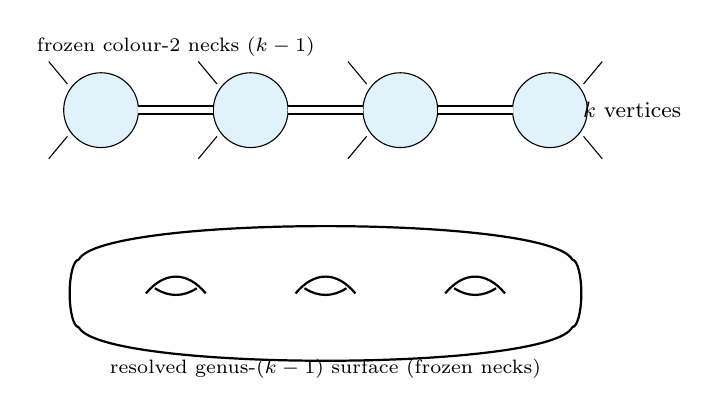
\begin{tikzpicture}[scale=0.95, every node/.style={font=\footnotesize}]
		\foreach \x in {0,2,4} {
			\filldraw[fill=SkyBlue!25, draw=black] (\x,1.3) circle (0.5);
			\draw (\x-0.45,1.65) -- (\x-0.7,1.95);
			\draw (\x-0.45,0.95) -- (\x-0.7,0.65);
		}
		\filldraw[fill=SkyBlue!25, draw=black] (6,1.3) circle (0.5);
		\draw (6+0.45,1.65) -- (6+0.7,1.95);
		\draw (6+0.45,0.95) -- (6+0.7,0.65);
		\foreach \x in {0,2,4} {
			\draw[double, double distance=2pt, thick] (\x+0.5,1.3) -- (\x+1.5,1.3);
		}
		\node at (7.1,1.3) {$k$ vertices};
		\node at (1,2.15) {\scriptsize frozen colour-2 necks ($k-1$)};
		\draw[thick] (-0.3,-0.7) .. controls (0,-0.1) and (6,-0.1) .. (6.3,-0.7);
		\draw[thick] (-0.3,-1.6) .. controls (0,-2.2) and (6,-2.2) .. (6.3,-1.6);
		\draw[thick] (-0.3,-0.7) arc (90:270:0.12 and 0.45);
		\draw[thick] (6.3,-0.7) arc (90:-90:0.12 and 0.45);
		\foreach \x in {1,3,5} {
			\draw[thick] (\x-0.4,-1.15) .. controls (\x-0.15,-0.85) and (\x+0.15,-0.85) .. (\x+0.4,-1.15);
			\draw[thick] (\x-0.28,-1.08) .. controls (\x-0.1,-1.2) and (\x+0.1,-1.2) .. (\x+0.28,-1.08);
		}
		\node at (3,-2.15) {\scriptsize resolved genus-$(k-1)$ surface (frozen necks)};
	\end{tikzpicture}
	\caption{\textbf{F2.} A length-$k$ chain of four-punctured spheres joined by
	$k-1$ frozen colour-2 necks (top), and the resolved genus-$(k-1)$ surface it
	stands for (bottom). The resolved handles are frozen and unpaid-for: the
	physical grading is that of the coloured tree (\Cref{rs:tab:grading}).}
	\label{rs:fig:chain}
\end{figure}

\begin{figure}[htp]
	\centering
	\begin{subfigure}[c]{0.48\linewidth}
		\centering
		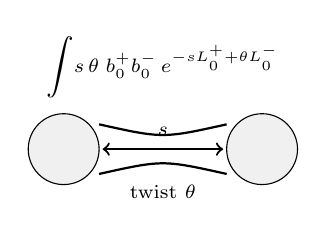
\begin{tikzpicture}[scale=0.9, every node/.style={font=\footnotesize}]
			\filldraw[fill=gray!12, draw=black] (-1.4,0) circle (0.5);
			\filldraw[fill=gray!12, draw=black] (1.4,0) circle (0.5);
			\draw[thick] (-0.9,0.35) .. controls (0,0.15) .. (0.9,0.35);
			\draw[thick] (-0.9,-0.35) .. controls (0,-0.15) .. (0.9,-0.35);
			\draw[<->, thick] (-0.85,0) -- (0.85,0);
			\node at (0,0.25) {\scriptsize $s$};
			\node at (0,-0.6) {\scriptsize twist $\theta$};
			\node at (0,1.15) {\scriptsize $\displaystyle\int\!\dd s\,\dd\theta\;b_0^+ b_0^-\,e^{-sL_0^+ + \I\theta L_0^-}$};
		\end{tikzpicture}
		\caption{Colour-1 edge \eqref{rs:eq:sewing}: a two-parameter cylinder family
		with two $b$-insertions. Geometric, propagating.}
		\label{rs:fig:kernels-a}
	\end{subfigure}
	\hfill
	\begin{subfigure}[c]{0.48\linewidth}
		\centering
		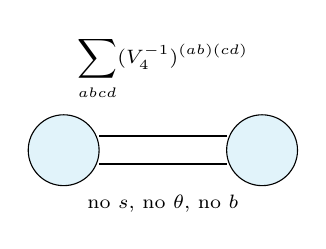
\begin{tikzpicture}[scale=0.9, every node/.style={font=\footnotesize}]
			\filldraw[fill=SkyBlue!25, draw=black] (-1.4,0) circle (0.5);
			\filldraw[fill=SkyBlue!25, draw=black] (1.4,0) circle (0.5);
			\draw[thick] (-0.9,0.2) -- (0.9,0.2);
			\draw[thick] (-0.9,-0.2) -- (0.9,-0.2);
			\node at (0,1.15) {\scriptsize $\displaystyle\sum_{abcd}(V_4^{-1})^{(ab)(cd)}$};
			\node at (0,-0.75) {\scriptsize no $s$, no $\theta$, no $b$};
		\end{tikzpicture}
		\caption{Colour-2 edge \eqref{rs:eq:c2insert}: a rigid two-strand state
		sandwich, no moduli, no $b$'s. Frozen, auxiliary.}
		\label{rs:fig:kernels-b}
	\end{subfigure}
	\caption{\textbf{F4.} The two internal kernels side by side
	(\Cref{rs:sec:kernels,rs:sec:operad}). The presence versus absence of the
	$(s,\theta)$ family and its $b$'s is the entire geometric distinction between
	propagating and auxiliary.}
	\label{rs:fig:kernels}
\end{figure}

\begin{figure}[htp]
	\centering
	\begin{tikzpicture}[scale=0.95, every node/.style={font=\footnotesize}]
		\filldraw[fill=SkyBlue!25, draw=black] (-1.7,0) ellipse (0.6 and 0.9);
		\filldraw[fill=SkyBlue!25, draw=black] (1.7,0) ellipse (0.6 and 0.9);
		\node at (-1.7,-1.25) {\scriptsize $\mc{V}_{0,6}$};
		\node at (1.7,-1.25) {\scriptsize $\mc{V}_{0,6}$};
		\foreach \y in {0.35,0,-0.35} {
			\draw[thick] (-1.1,\y) -- (1.1,\y);
		}
		\node at (0,0.95) {\scriptsize colour-3 cable ($3$ strands, $G_3^{-1}$)};
		\foreach \y in {0.5,0,-0.5} {
			\draw (-2.25,\y) -- (-2.7,\y);
			\draw (2.25,\y) -- (2.7,\y);
		}
		\draw[-{Latex}, thick] (0,-1.7) -- (0,-2.3);
		\begin{scope}[yshift=-3.4cm]
			\draw[thick] (-2.2,0.55) .. controls (-2,1.05) and (2,1.05) .. (2.2,0.55);
			\draw[thick] (-2.2,-0.55) .. controls (-2,-1.05) and (2,-1.05) .. (2.2,-0.55);
			\draw[thick] (-2.2,0.55) arc (90:270:0.12 and 0.55);
			\draw[thick] (2.2,0.55) arc (90:-90:0.12 and 0.55);
			\foreach \x in {-0.9,0.9} {
				\draw[thick] (\x-0.4,-0.05) .. controls (\x-0.15,0.28) and (\x+0.15,0.28) .. (\x+0.4,-0.05);
				\draw[thick] (\x-0.28,0.02) .. controls (\x-0.1,-0.12) and (\x+0.1,-0.12) .. (\x+0.28,0.02);
			}
			\node at (0,-0.95) {\scriptsize resolved genus-$2$ surface (frozen)};
		\end{scope}
	\end{tikzpicture}
	\caption{\textbf{F3.} A single colour-3 cable ($3$ strands, contraction
	$G_3^{-1}$) between two dressed six-punctured vertex regions, and the resolved
	genus-$2$ surface it stands for: $g_{\rm res}=k-1=2$ from \eqref{rs:eq:genus},
	physical genus $0$. See \Cref{rs:sec:tower}.}
	\label{rs:fig:cable}
\end{figure}

\begin{figure}[htp]
	\centering
	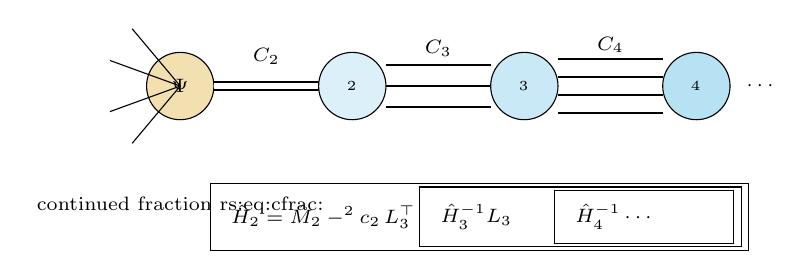
\begin{tikzpicture}[scale=0.95, every node/.style={font=\footnotesize}]
		\filldraw[fill=Goldenrod!35, draw=black] (0,0) circle (0.45);
		\node at (0,0) {\scriptsize $\Psi$};
		\foreach \a in {200,230,160,130} { \draw (0,0) -- (\a:1.0); }
		\draw[double, double distance=2pt, thick] (0.45,0) -- (1.85,0);
		\filldraw[fill=SkyBlue!30, draw=black] (2.3,0) circle (0.45);
		\node at (2.3,0) {\scriptsize $\Sig_2$};
		\node at (1.15,0.4) {\scriptsize $C_2$};
		\foreach \y in {0.28,0,-0.28} { \draw[thick] (2.75,\y) -- (4.15,\y); }
		\filldraw[fill=SkyBlue!45, draw=black] (4.6,0) circle (0.45);
		\node at (4.6,0) {\scriptsize $\Sig_3$};
		\node at (3.45,0.5) {\scriptsize $C_3$};
		\foreach \y in {0.36,0.12,-0.12,-0.36} { \draw[thick] (5.05,\y) -- (6.45,\y); }
		\filldraw[fill=SkyBlue!60, draw=black] (6.9,0) circle (0.45);
		\node at (6.9,0) {\scriptsize $\Sig_4$};
		\node at (5.75,0.55) {\scriptsize $C_4$};
		\node at (7.75,0) {\scriptsize $\cdots$};
		\begin{scope}[yshift=-2.2cm]
			\node at (0,0.6) {\scriptsize continued fraction \eqref{rs:eq:cfrac}:};
			\draw (0.4,0) rectangle (7.6,0.9);
			\node[anchor=west] at (0.55,0.45) {\scriptsize $\hat H_2=\hat M_2-\gs^2 c_2\,L_3^\top$};
			\draw (3.2,0.05) rectangle (7.5,0.85);
			\node[anchor=west] at (3.35,0.45) {\scriptsize $\hat H_3^{-1}L_3$};
			\draw (5.0,0.1) rectangle (7.4,0.8);
			\node[anchor=west] at (5.15,0.45) {\scriptsize $\hat H_4^{-1}\cdots$};
		\end{scope}
	\end{tikzpicture}
	\caption{\textbf{F5.} The scheme-B tower as a coloured tree: cables of
	increasing strand number $C_2,C_3,C_4,\dots$ (\Cref{rs:eq:colours}), with the
	continued fraction \eqref{rs:eq:cfrac} as nested boxes (each $\hat H_{k+1}^{-1}$
	sandwiched between $L_{k+1}$'s). Everything is a tree in the coloured grading;
	the nesting telescopes to contact support.}
	\label{rs:fig:tower}
\end{figure}


